\documentclass{article}
\usepackage[utf8x]{inputenc}
\usepackage[english,russian]{babel}
\usepackage{graphicx}
\usepackage{todonotes}
\usepackage{hyperref}
\usepackage{caption}
\usepackage{bm}
\usepackage{amsmath}
\usepackage{subcaption}

\newcommand  {\figref  } [1]     {рис.~\ref{#1}}
\newcommand  {\figrefp } [1]     {(\figref{#1})}
\newcommand  {\op      } [1]     { \bm{#1}           }
\renewcommand{\vec     } [1]     { \bm{#1}           }
\newcommand  {\vr      }         { \vec{r}           }
\newcommand  {\vR      }         { \vec{R}           }
\newcommand  {\paren   } [1]     { \left( #1 \right) }
\def          \fun       _#1(#2) { #1 \paren{#2}     }
\newcommand  {\inv     } [1]     { \frac{1}{#1}      }
\def          \pdsqr     _#1_#2  { \frac{\partial^2}{\partial #2^2}#1 }
\newcommand  {\dsr   } { \fun_{\Delta s^2}(\vr) }
\newcommand  {\rmR   } { \vr - \vR }
\newcommand  {\rmrz  } { \vr - \vec{r}_0 }
\newcommand  {\rmrw  } { \vr - \tilde{\vec{r}} }
\newcommand  {\Rmrw  } { \vR - \tilde{\vec{r}} }
\newcommand  {\armR  } { \left| \rmR  \right| }
\newcommand  {\armrw } { \left| \rmrw \right| }
\newcommand  {\aRmrw } { \left| \Rmrw \right| }
\newcommand  {\armrz } { \left| \rmrz \right| }
\renewcommand{\L     } { \fun_L(\vR,t|\vr) }

\begin{document}
\title{Изучение методов сейсмической миграции на примере волнового уравнения}
\author{\textbf{Голубев В.И., Войнов О.Я.} \\ Лаборатория прикладной вычислительной геофизики МФТИ}
\maketitle

\section{Введение}

Одним из методов поиска и разведки месторождений полезных ископаемых, таких как нефть и природный газ, является сейсморазведка.
Её основа - распространение упругих волн в геологических средах, а также их отражение от неоднородностей.
Как правило, в качестве источника сигнала используется взрывчатое вещество, расположенное на дневной поверхности.
Для регистрации сигнала используются сейсмоприёмники - специальные устройства, регистрирующие движения поверхности.

В дальнейшем на основе обработки накопленных данных делаются выводы о внутреннем строении геологической среды (мощности пластов,
зоны трещиноватости, границы резервуара).
При этом принято различать две задачи такой обработки: определение положения отражающих горизонтов (миграция) и восстановление скоростной модели среды (инверсия).

Перед авторами отчёта были поставлены следующие научно-технические задачи:
\begin{itemize}
\item изучение методов сейсмической миграции на примере волнового уравнения;
\item разработка вычислительного алгоритма и компьютерной программы миграции на основе интегральной формулы Кирхгофа;
\item разработка вычислительного алгоритма и компьютерной программы миграции на основе сопряженного оператора для волнового уравнения;
\item сравнительный анализ двух алгоритмов на простых моделях.
\end{itemize}

Все задачи были выполнены.

Лидер проекта – Василий Голубев.
Рекомендуемые руководителем лаборатории разделы книги “Geophysical inverse theory and regularization problems” - раздел 15.4 стр 503 - 516.

\section{Используемые обозначения}

Для ясности опишем кратко использованные и разработанные программные продукты.

KirScal - программа для расчёта интеграла Кирхгофа в трёхмерной постановке для волнового уравнения (однородная среда). Предполагается, что на верхней границе полупространства задаётся произвольный источник. Производится построение волнового поля в заданный момент времени. Разработана Голубевым В.И.

AcInverse - программа для построения миграционного изображения (волновое уравнение) с использованием формулы Кирхгофа (приближение Рэлея).
Разработана Голубевым В.И.

Borni - программа для решения прямой задачи (волновое уравнение) и построения миграционного изображения на основе подхода с присоединённым оператором.
При этом матрица связи наблюдений и параметров модели получена с использованием приближения Борна.
Разработана Войновым О.Я.

Madagascar - OpenSource комплекс для моделирования/обработки данных сейсмической разведки.
Включает широкий спектр программ, как для прямого моделирования и построения синтетических сейсмограмм, так и для решения обратных задач (миграция, инверсия).
Разработка начата в 2003 году, проект актуален (например, Workshop August 2014).

\section{Теория}

Динамическое поведение акустической среды (распределение отклонения давления в ней от стационарного значения)
может быть описано следующим волновым уравнением (\cite{Zhdanov_2007}, 13.54):
\begin{equation}
\label{wave_equation}
\nabla^2P(\vec{r},t) - \frac{1}{c^2(\vec{r})}\frac{\partial^2}{\partial t^2}
	P(\vec{r},t) = - F^e(\vec{r},t),
\end{equation}

где - $P(\vec{r},t)$ - поле давления, $F^e(\vec{r},t)$ - напряжение внешнего источника, $c(\vec{r})$
- скорость распространения волны в среде.

\subsection{Решение прямой задачи. Интеграл Кирхгофа}

Рассмотрим задачу о воздействии динамического источника на поверхность некоторого объёма среды.
В этом случае значение давления во внутренней точке области $\vec{r'}$ в момент времени $t'$ может быть выражено следующей формулой (\cite{Zhdanov_2007}, 13.112):
\begin{equation}
\label{eq_kirchhoff_common}
P(\vec{r'}, t') = \int_S \int_{-\infty}^{+\infty} [G^w(\vec{r'}, t' | \vec{r}, t) \frac{\partial}
{\partial n} P(\vec{r}, t) - P(\vec{r}, t) \frac{\partial}{\partial n} G^w(\vec{r'}, t' |
\vec{r}, t)] dt ds,
\end{equation}

где интеграл берётся по поверхности, ограничивающей объём, а функция $G^w(\vec{r'}, t' | \vec{r}, t)$ называется функцией Грина и является решением уравнения \ref{wave_equation} для случая внешнего воздействия в виде дельта-функции.

Пусть $c(\vec{r'}) = const$, т.е. среда является изотропной.
Тогда функция Грина может быть получена аналитически (\cite{Zhdanov_1988}, 4.13):
\begin{equation}
\label{eq_grin_function}
G^w(\vec{r}, t | \vec{r'}, t') = \frac{1}{4\pi|\vec{r} - \vec{r'}|}\delta(t - t' - \frac{|\vec{r} -
\vec{r'}|}{c}),
\end{equation}
где $\vec{r'}, t'$ - место расположения источника и время, в которое он начал действовать.

Подставляя в (\ref{eq_kirchhoff_common}) выражение для функции Грина в явном виде (\ref{eq_grin_function}) получим
\begin{equation}
\label{eq_kirchhoff_homogeneous}
P(\vec{r'}, t') = \frac{1}{4\pi} \int_S [\frac{1}{c|\vec{r'} - \vec{r}|}
\frac{\partial |\vec{r'} - \vec{r}|}{\partial n}\frac{\partial P'}{\partial t'}
- \frac{\partial}{\partial n}(\frac{1}{|\vec{r'} - \vec{r}|}) P' + 
\frac{1}{|\vec{r'} - \vec{r}|}\frac{\partial}{\partial n}P'] ds,
\end{equation}
где $P' = P(\vec{r}, t' - \frac{|\vec{r'} - \vec{r}|}{c})$.
 
Для задач сейсмики актуальна задача о распространении сейсмических волн в полупространстве (от дневной поверхности вниз и обратно после отражения от неоднородностей).
При такой постановке $\frac{\partial}{\partial n} = -\frac{\partial}{\partial z}$, поэтому выражение (\ref{eq_kirchhoff_homogeneous}) может быть упрощено до вида:
\begin{equation}
\label{eq_kirchhoff_final}
P(\vec{r'}, t') = \frac{1}{4\pi} \int_S [\frac{z' - z}{|\vec{r'} - \vec{r}|}(\frac{1}{c}
\frac{\partial P'}{\partial t'} + \frac{1}{|\vec{r'} - \vec{r}|^2} P') - \frac{1}{|\vec{r'}
- \vec{r}|}\frac{\partial P'}{\partial z}] ds
\end{equation}

Пусть, например, дополнительно известна функция источника (импульс Риккера):
\begin{equation}
\label{eq_ricker_wavelet}
P_{ricker} = P_0(1-2 \pi^2f^2t^2)e^{-\pi^2f^2t^2}.
\end{equation}

Тогда могут быть явно вычислены производные, стоящие в выражении (\ref{eq_kirchhoff_final}):
\begin{equation}
\label{eq_dp'_dt'}
\frac{\partial P'}{\partial t'} = -2\pi^2f^2P_0(3-2 \pi^2f^2(t' - \frac{|\vec{r'} - \vec{r}|}{c})^2)e^{-\pi^2f^2(t' - \frac{|\vec{r'} - \vec{r}|}{c})^2},
\end{equation}
и
\begin{equation}
\label{eq_dp'_dz}
\frac{\partial P'}{\partial z} = -2\pi^2f^2P_0(t' - \frac{|\vec{r'} - \vec{r}|}{c})[3-2 \pi^2f^2(t' - \frac{|\vec{r'} - \vec{r}|}{c})^2]e^{-\pi^2f^2(t' - \frac{|\vec{r'} - \vec{r}|}{c})^2}
\frac{z'-z}{c|\vec{r'}-\vec{r}|},
\end{equation}
а функция $P'(\vec{r'}, t')$ может быть записана в виде:
\begin{equation}
\label{eq_surface_pressure}
P'(\vec{r'}, t') = P(\vec{r}, t' - \frac{|\vec{r'} - \vec{r}|}{c}) = P_0(1-2 \pi^2f^2(t' - \frac{|\vec{r'} - \vec{r}|}{c})^2)e^{-\pi^2f^2(t'-\frac{|\vec{r'} - \vec{r}|}{c})^2}.
\end{equation}

\subsection{Миграция. Интеграл Кирхгофа.}

	Задачу сейсмической миграции можно сформулировать следующим образом. Пусть в некоторой области над земной поверхностью расположено множество сейсмоприемников, на каждом из которых измерено значение скалярного волнового поля для определенного набора отсчетов по времени. Требуется определить положение отражающих границ внутри земной среды под данной областью для некоторого диапазона глубин. Традицонную сейсмическую миграцию также можно рассматривать как первую итерацию в полном решении обратной задачи сейсморазведки, для которого требуется найти распределение скорости распространения волнового поля в исследуемой области \cite{tarantola2005}.

В рамках сформулированных задач были произведены расчеты для классической модели Marmousi \figrefp{marmousi}. Для этого был разработан вычислительный алгоритм на основе метода присоединенного оператора и приближения Борна. Приведем математическое обоснование этого метода \cite{Zhdanov_2007},\; \cite{claerbout2004}.
В книге \cite{Zhdanov_2007} изложена теория, позволяющая рассчитать пространственное распределение скалярного параметра $U^m(\vec{r'})$, высокие значения которого соответствуют
месту расположения отражающего горизонта.
Для случая горизонтальной плоскости наблюдения расчётная формула представима в виде (\cite{Zhdanov_2007}, 15.208):
\begin{equation}
\label{rayleigh_migration}
U^m(\vec{r'}) = -\frac{1}{2\pi}\frac{\partial}{\partial z'}
	\int_S \frac{P(\vec{r},\frac{2|\vec{r'}-\vec{r}|}{c})}{|\vec{r'}-\vec{r}|}ds,
\end{equation}
где $\vec{r}$ - координата на поверхности, в которой записывается сейсмограмма, $\vec{r'}$ - координата в объёме, где ищется мигрированное изображение, $c$ - скорость распространения волн.

\subsection{Миграция. Приближение Борна.}

Прямая задача сейсморазведки может быть представлена в виде
\begin{equation} \label{dLm}
\vec d = \op L \vec m .
\end{equation}
Здесь $\vec d$ -- наблюдаемые на сейсмоприемниках данные, $\vec m$ -- параметры среды, $\op L$ -- оператор прямой задачи. Миграционное изображение среды задается выражением \cite{claerbout2004}
\begin{equation}
\vec m_{migr} = \op L^* \vec d .
\end{equation}
а средне-квадратичная модель (\cite{Zhdanov_2007}, 3.9) --
\begin{equation} \label{m_0}
\vec m_0 = \left( \op L^* \op L \right)^{-1} \vec m_{migr} ,
\end{equation}
Присоединенный оператор $\op L^*$ определяется как
\begin{equation}
\left(\vec d, \op L \vec m \right) = \left( \op L^* \vec d, \vec m \right),\quad \forall \vec m,\vec d ,
\end{equation}
где круглыми скобками обозначено скалярное произведение.

Рассмотрим акустическую среду. В ней скалярное волновое поле $p$ удовлетворяет уравнению Гельмгольца (\cite{Zhdanov_2007}, 13.56)
\begin{equation}
\nabla^2 \fun_p(\vr,\omega) + \omega^2 \fun_s^2(\vr) \fun_p(\vr,\omega) = - \fun_f(\vr,\omega) ,
\end{equation}
где $f$ -- напряжение внешнего источника энергии, $s$ -- медленность волны, которую представим в виде $ \fun_s^2(\vr) = \fun_s_b^2(\vr) + \dsr $, а $s_b$ назовем фоновой медленностью. Пусть первичное поле $p^i$ есть известное решение уравнения Гельмгольца с фоновой медленностью
\begin{equation}
\nabla^2 \fun_p^i(\vr,\omega) + \omega^2 \fun_s_b^2(\vr) \fun_p^i(\vr,\omega) = - \fun_f(\vr,\omega) .
\end{equation}
Тогда вторичное поле $p^s = p - p^i$ удовлетворяет уравнению
\begin{equation}
\nabla^2 \fun_p^s(\vr,\omega) + \omega^2 \fun_s_b^2(\vr) \fun_p^s(\vr,\omega) = - \omega^2 \dsr \fun_p(\vr,\omega) .
\end{equation}
Если медленность среды непостоянна лишь в некоторой ограниченной области $\fun_s(\vr) = s_b = const ,\, \vr \not\in D$, то решение последнего уравнения на границе этой области иммеет вид (\cite{Zhdanov_2007}, 14.19)
\begin{equation}
\fun_p^s(\vR,\omega) = \omega^2 \int_{\vr\in D} \frac{e^{i \omega s_b \armR} }{4\pi \armR}  \dsr \fun_p(\vr,\omega) dV.
\end{equation}
В том случае, когда по сравнению с первичным полем вторичным можно пренебречь, получаем приближение Борна
\begin{equation} \begin{gathered} \label{Born}
\fun_p^s(\vR,\omega) \simeq \omega^2 \int_{\vr\in D} \frac{e^{i \omega s_b \armR} }{4\pi \armR} \dsr \fun_p^i(\vr,\omega) dV, \\
\fun_p^s(\vR,t)      \simeq -        \int_{\vr\in D} \frac{\dsr}                   {4\pi \armR} \pdsqr_{\fun_p^i(\vr,t - s_b\armR)}_t dV.
\end{gathered} \end{equation}

Пусть источник возмущения -- точечный импульс Рикера, возникающий в нулевой момент времени в точке $\vec r_0$ \figrefp{ricker}: 
\begin{equation} \label{10}
\fun_p^i(\vr,t) = \inv{4 \pi \armrz } \fun_RW( t - s_b \armrz ) ,
\end{equation}
где
\begin{equation} \label{eq:ricker}
RW(t) = \left( 1 - 2 \pi^2 f_M^2 t^2 \right) e^{- \pi^2 f_M^2 t^2}.
\end{equation}
\begin{figure}[tb]
\centering
\begin{subfigure}{.3333\textwidth}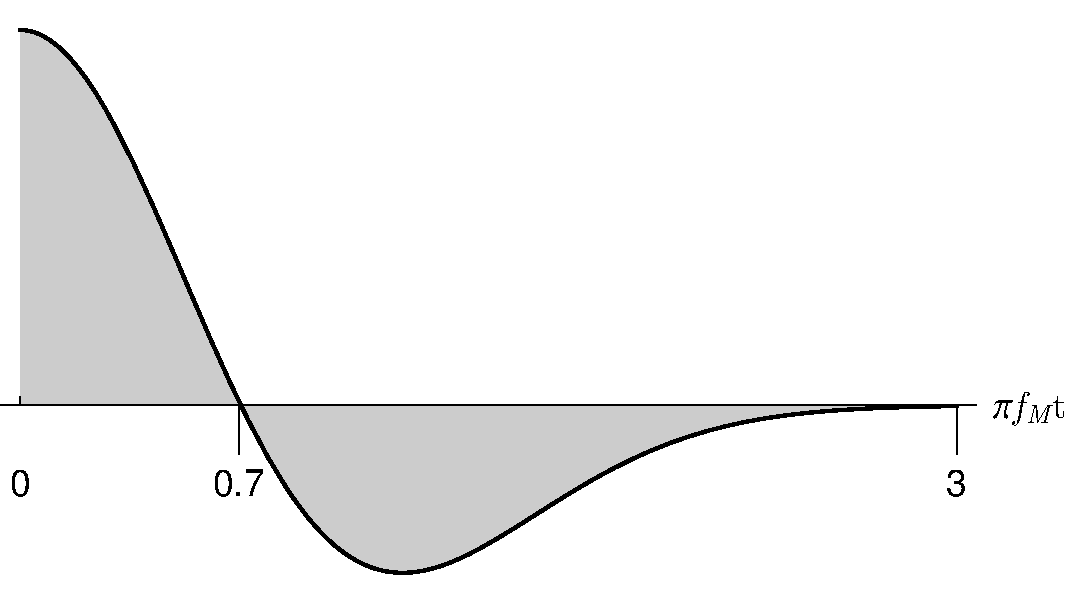
\includegraphics[width=\textwidth]{pic/report_april/ricker}\caption{график функции $RW(t)$}\end{subfigure}\hspace{.1111\textwidth}
\begin{subfigure}{.3333\textwidth}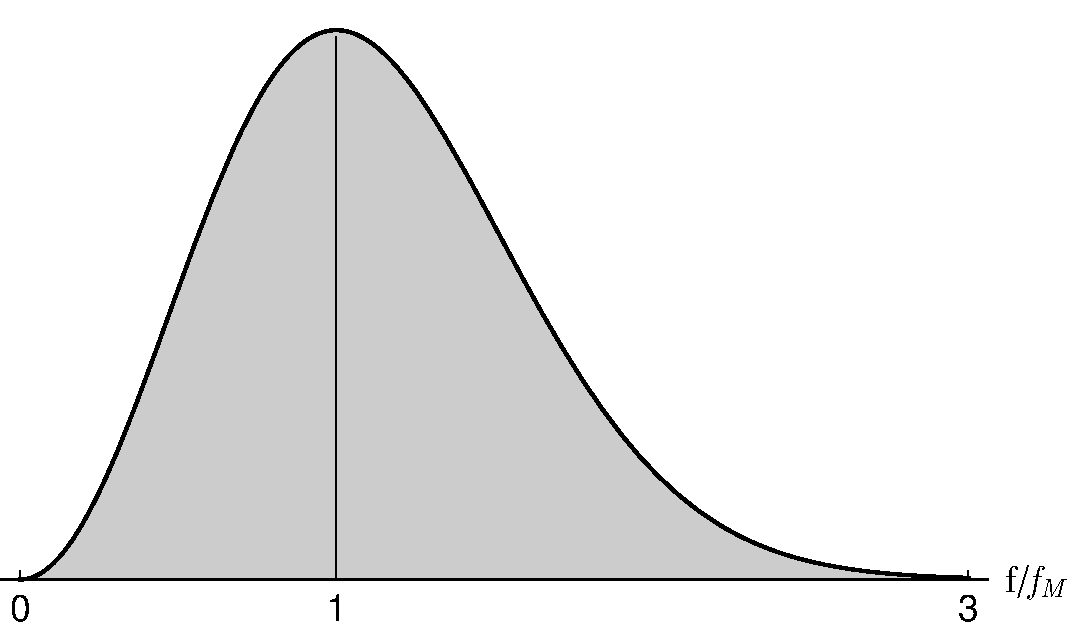
\includegraphics[width=\textwidth]{pic/report_april/rickeromega}\caption{Фурье-преобразование функции $RW(t)$}\end{subfigure}%i
\caption{} \label{ricker}
\end{figure}
Тогда 
\begin{equation}
\fun_p^s(\vR,t) = \int_{\vr\in D} \frac{ f_M^2 }{ 2 \armR \armrz } e^{ -\tau^2 } \left( \tau^4 - 3 \tau^2 + \frac{3}{4} \right) \dsr dV ,
\end{equation}
где $\tau = \pi f_M \left( t - s_b \armR - s_b \armrz \right)$.

Будем рассматривать далее случай "нулевого удаления" (zero-offset) источника возмущения от приемника $\left( \vec r_0 = \vec R \right)$
\begin{equation} \label{eq:13}
\fun_p^s(\vR,t) = \int_{\vr\in D} \frac{ f_M^2 }{ 2 \left( \rmR \right)^2 } e^{ -\tau^2 } \left( \tau^4 - 3 \tau^2 + \frac{3}{4} \right) \dsr dV ,
\end{equation}
и $\tau = \pi f_M \left( t - 2 s_b \armR \right)$. В соответствии с полученным выражением оператор прямого моделирования $\op L$ имеет вид
\begin{equation} \label{th_1}
\fun_d(\vR,t) = \fun_L(\vR,t|\vr) \fun_m(\vr) = \int_{\vr\in D} \frac{ f_M^2 }{ 2 \left( \rmR \right)^2 } e^{ -\tau^2 } \left( \tau^4 - 3 \tau^2 + \frac{3}{4} \right) \fun_m(\vr) dV ,
\end{equation}
а сопряженный к нему оператор $\op L^*$ --
\begin{equation} \label{th_2}
\fun_m(\vR) = \fun_L^*(\vR|\vr,t) \fun_d(\vr, t) = \int_{t_{min}}^{t_{max}} \int_{\vr\in S} \frac{ f_M^2 }{ 2 \left( \rmR \right)^2 } e^{ -\tau^2 } \left( \tau^4 - 3 \tau^2 + \frac{3}{4} \right) \fun_d(\vr,t) dS dt ,
\end{equation}
где $S$ -- принажлежит границе области $G$, а $\left(t_{min},t_{max}\right)$ -- некоторый временной диапазон.

\section{Численное моделирование}

\subsection{Решение прямой задачи. Интеграл Кирхгофа}

Была разработана программа KirScal на языке Python, которая вычисляет численно интеграл (\ref{eq_kirchhoff_final}) методом прямоугольников с подстановкой (\ref{eq_dp'_dt'} и \ref{eq_dp'_dz}).
Проведён расчёт с $C_P = 2000$ м/с, импульс Риккера с $f = 50$ Гц.
На рисунках (\ref{img_point_1} - \ref{img_point_3}) представлены волновые картины при воздействии точечного источника.
Как видно, происходит распространение сферической волны от места расположения источника вглубь среды.

\noindent
\begin{minipage}{\linewidth}
\makebox[\linewidth]{
  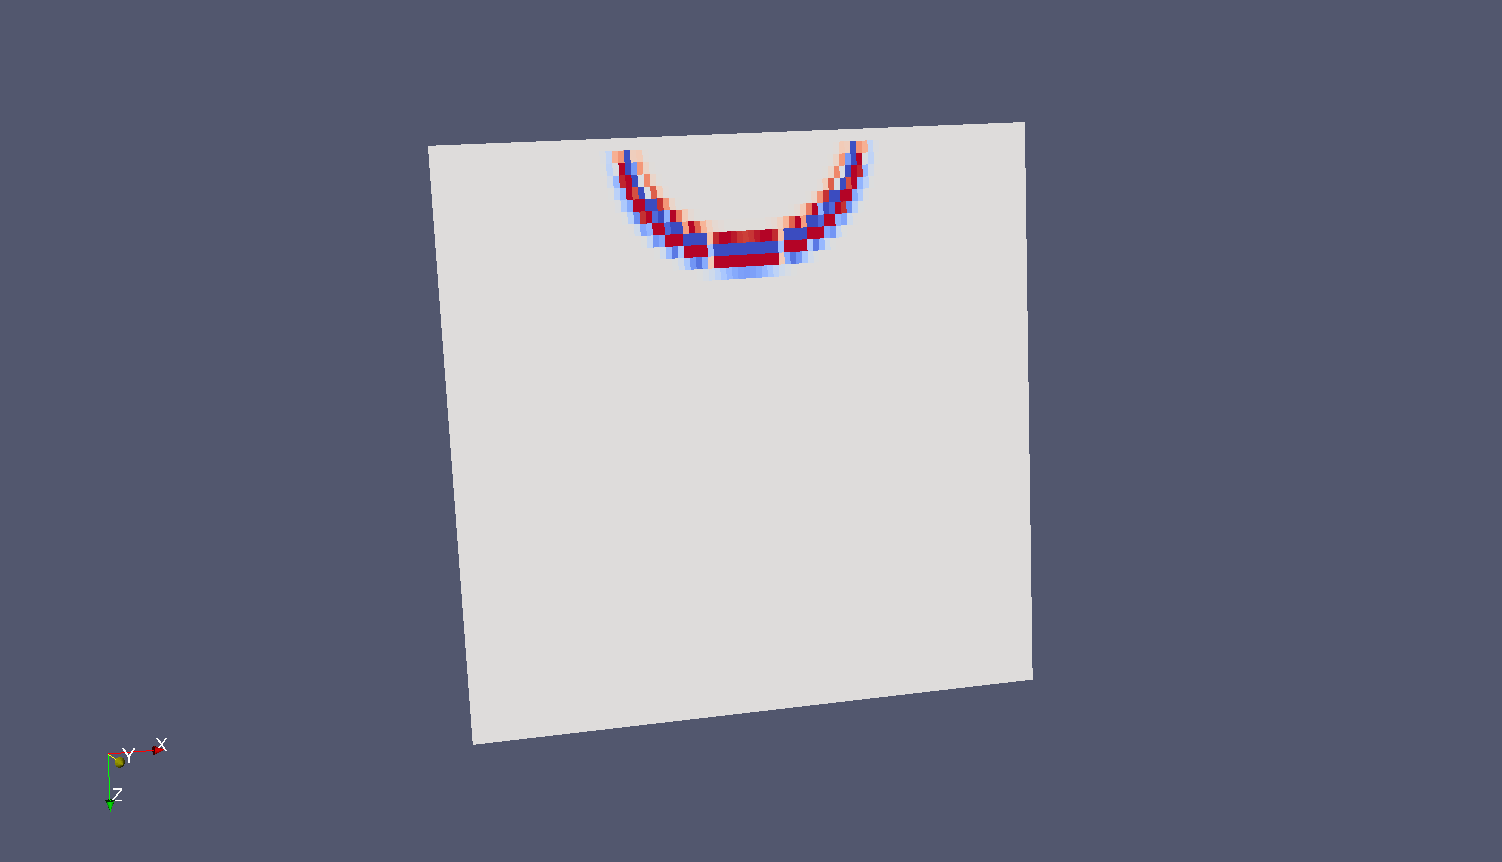
\includegraphics[scale=0.2]{pic_kirchhoff_scalar/point_1.png}
}
\captionof{figure}{Распределение давления по области через 100 мс}
\label{img_point_1}
\end{minipage}

\noindent
\begin{minipage}{\linewidth}
\makebox[\linewidth]{
    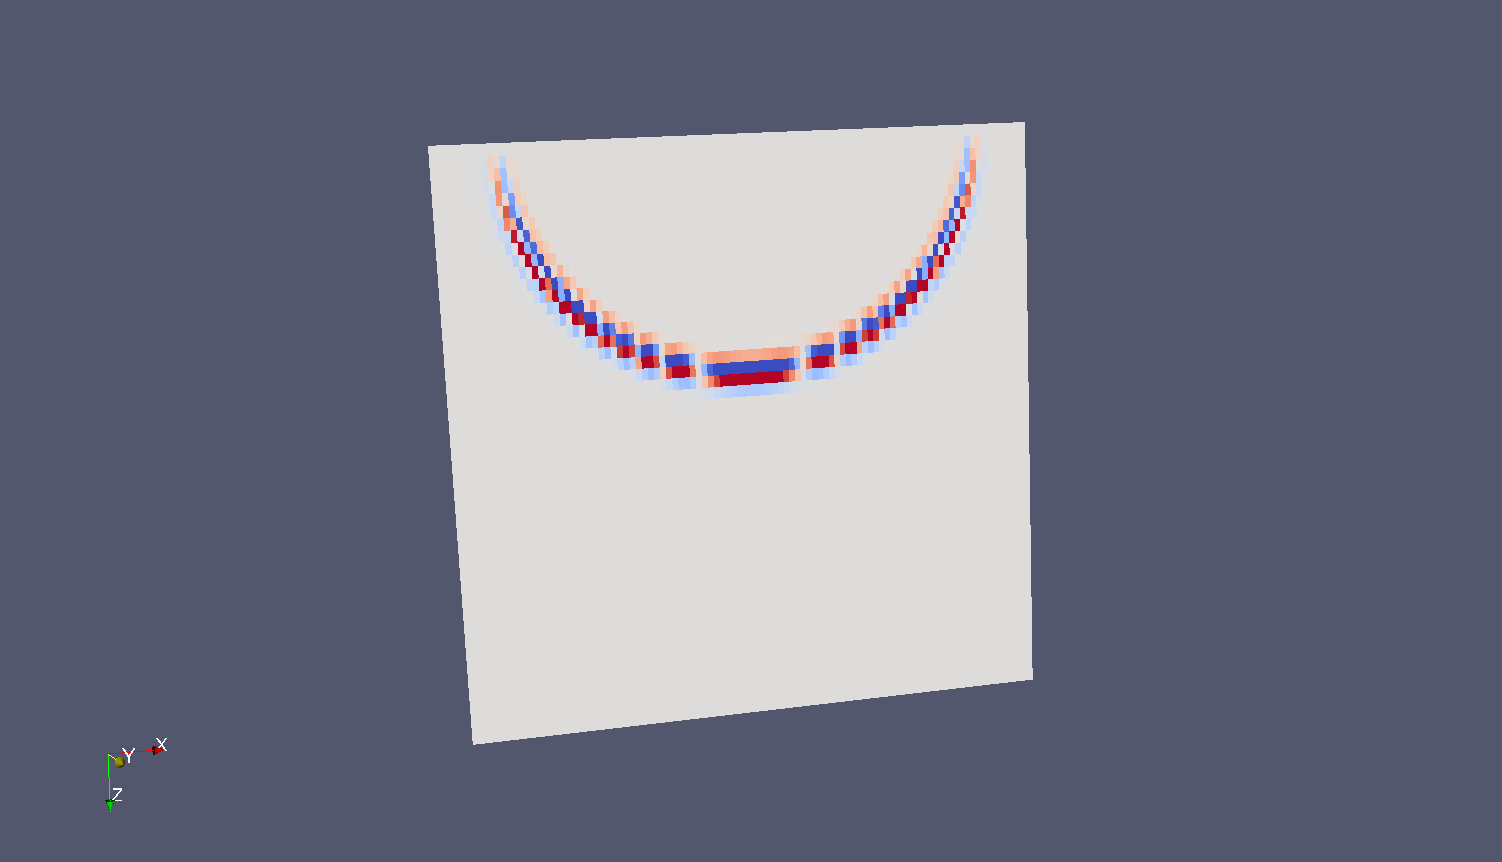
\includegraphics[scale=0.2]{pic_kirchhoff_scalar/point_2.png}
}
\captionof{figure}{Распределение давления по области через 200 мс}
\label{img_point_2}
\end{minipage}

\noindent
\begin{minipage}{\linewidth}
\makebox[\linewidth]{
  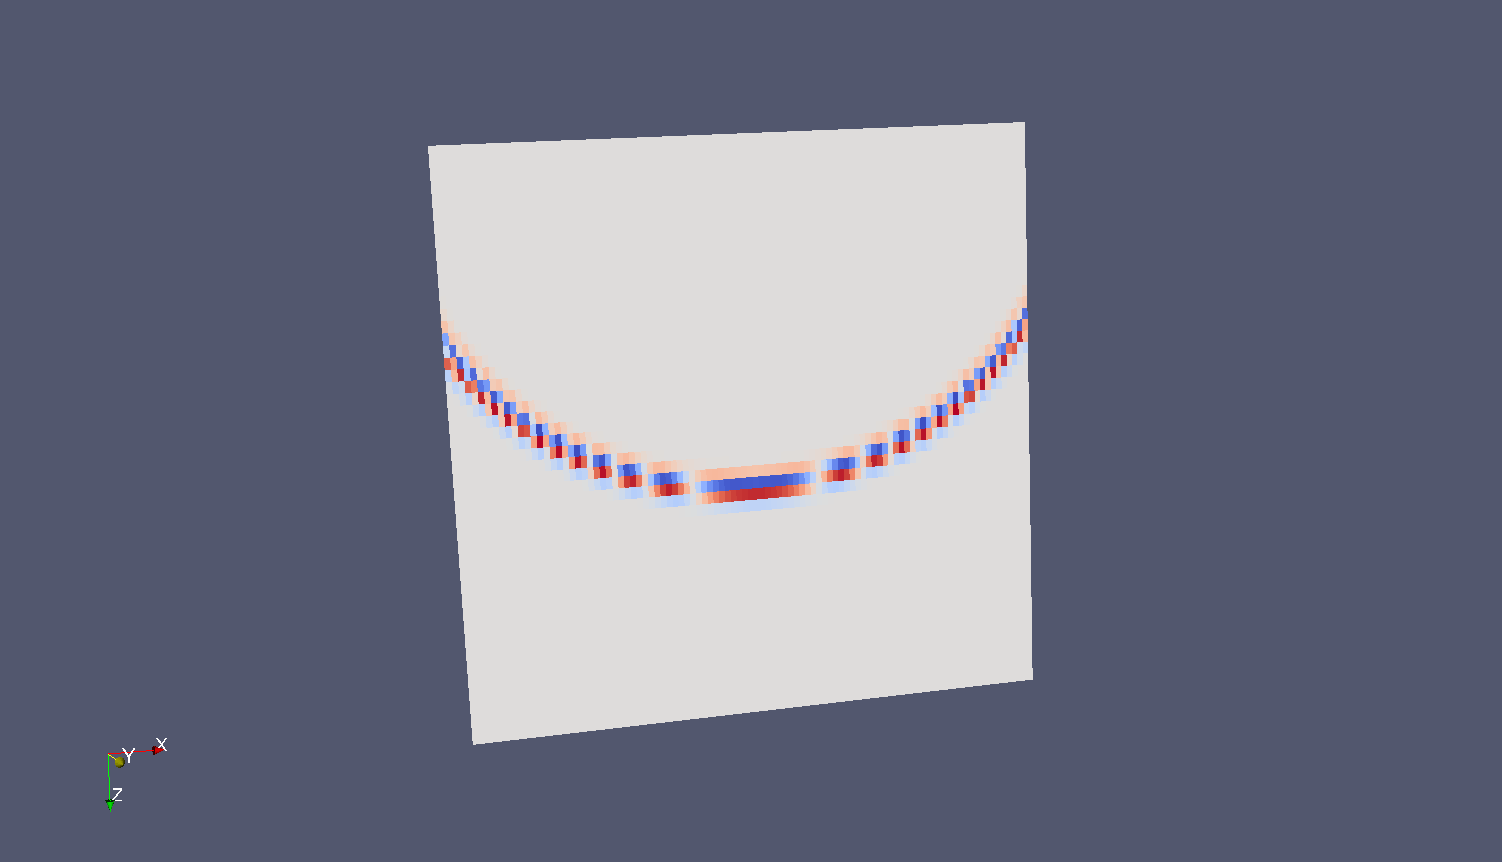
\includegraphics[scale=0.2]{pic_kirchhoff_scalar/point_3.png}
}
\captionof{figure}{Распределение давления по области через 300 мс}
\label{img_point_3}
\end{minipage}

\subsection{ПО Madagascar.}

Существует несколько программных комплексов, ориентированных на моделирование сейсмических процессов.
К ним относятся, например, Madagascar (www.ahay.org), Seismic Unix (www.seismicunix.com) и т.д.
В ходе выполнения исследовательской работы был частично освоен Madagascar.
Остановимся на одной его программе, называющейся sfkirmod.
С её помощью можно получать синтетические сейсмограммы для геологической среды (2D, для 3D можно использовать sfkirmod3) в акустическом приближении с:
- постоянной скоростью распространения волн, - постоянным градиентом скорости, - постоянным градиентом квадрата скорости.
Алгоритм работы программы основан на статье \cite{Haddon_1981}.

Для иллюстрации работы sfkirmod был проведён расчёт распространения сейсмического сигнала в однородной модели среды со скоростью 2500 м/с размерами 10 км x 5 км при
наличии отражающей границы на глубине 2,5 км.
На рисунке \ref{seismo_1} показана сейсмограмма для следующей расстановки: 1 источник в точке (0, 5), 2001 приёмник слева направо вдоль всех 10 км модели с интервалом 5 м.
Функция источника - Риккер 25 Гц.

\noindent
\begin{minipage}{\linewidth}
\makebox[\linewidth]{
  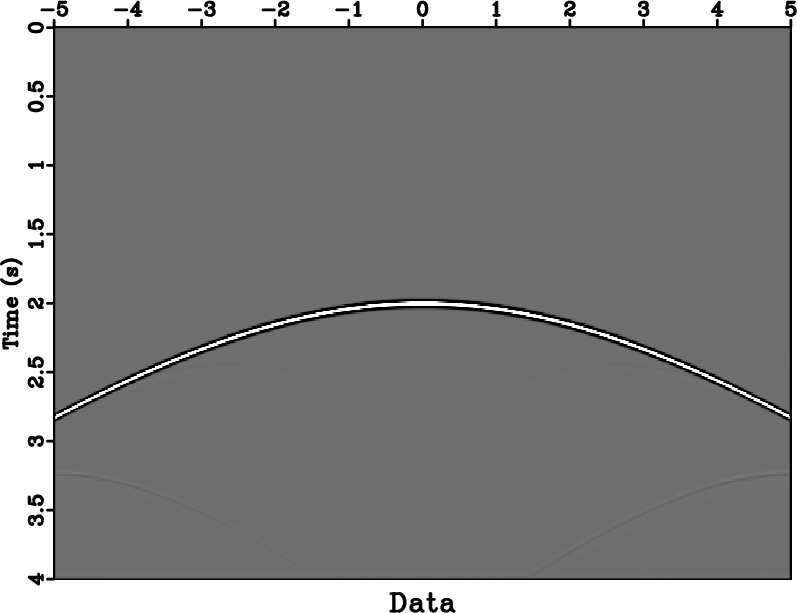
\includegraphics[scale=0.3]{./pic/report_april/Figure_1.png}
}
\captionof{figure}{Сейсмограмма с одной прямой границей.}
\label{seismo_1}
\end{minipage}

Также имеется возможность построения Zero-Offset сейсмограммы, т.е. когда каждая сейсмотрасса получена в условиях совпадения координат источника и приёмника.
На рисунке \ref{seismo_2} показана ZO-сейсмограмма для той же самой модели среды.
Использовался 2001 источник-приёмник с интервалом 50 м на всё протяжении расчётной области.

\noindent
\begin{minipage}{\linewidth}
\makebox[\linewidth]{
  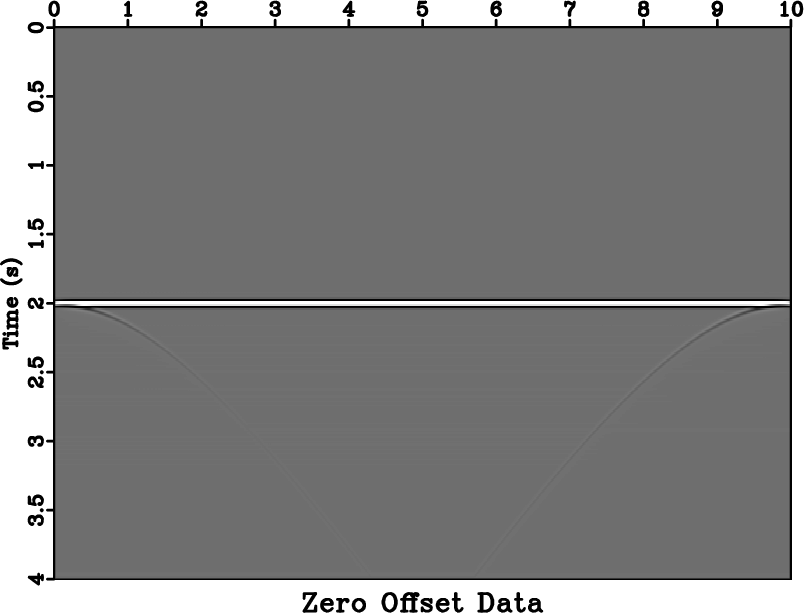
\includegraphics[scale=0.3]{./pic/report_april/Figure_2.png}
}
\captionof{figure}{ZO-cейсмограмма с одной прямой границей.}
\label{seismo_2}
\end{minipage}

При этом программа kirmod позволяет получить синтетическую сейсмограмму для произвольного распределения отражающих границ в пространстве.
Их можно задавать аналитическими функциями.
Для примера была рассчитана модель среды с тремя отражающими горизонтами, два из которых криволинейные.
Границы задавались функциями $x_2 = (3.0 - 0.1 * x_1)$, $x_2 = 0.5 * e^{\frac{(x_1 - 5.0)^2}{25}} - 0.4$ и $x_2 = -3.8 + 0.1 * x_1 + e^{\frac{(x_1 - 5.0)^2}{25}}$ соответственно.
При этом обозначены $x_1$ - горизонтальная ось, $x_2$ - вертикальная ось.
Параметры расстановки выбирались аналогично предыдущему расчёту.
Результаты расчётов представлены на рисунках \ref{seismo_3} - \ref{seismo_4}.

\noindent
\begin{minipage}{\linewidth}
\makebox[\linewidth]{
  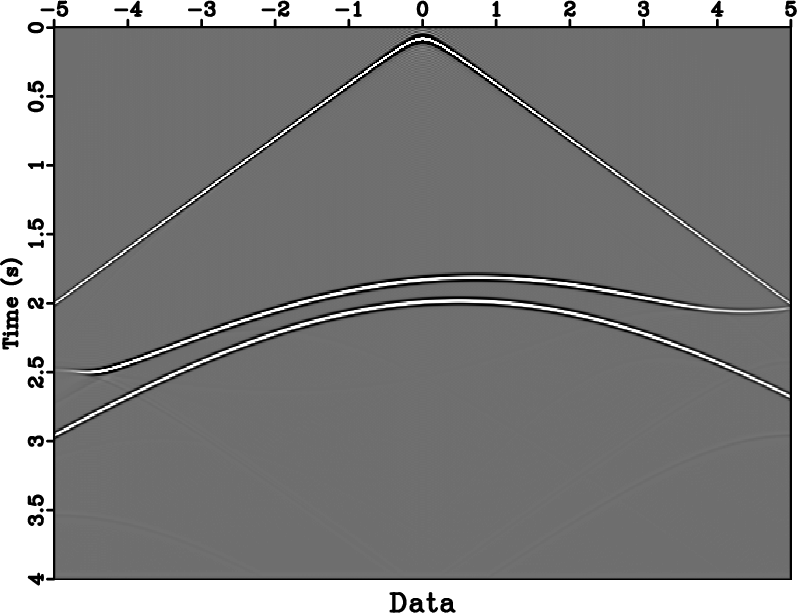
\includegraphics[scale=0.3]{./pic/report_april/Figure_3.png}
}
\captionof{figure}{Сейсмограмма для модели с тремя отражающими горизонтами.}
\label{seismo_3}
\end{minipage}

\noindent
\begin{minipage}{\linewidth}
\makebox[\linewidth]{
  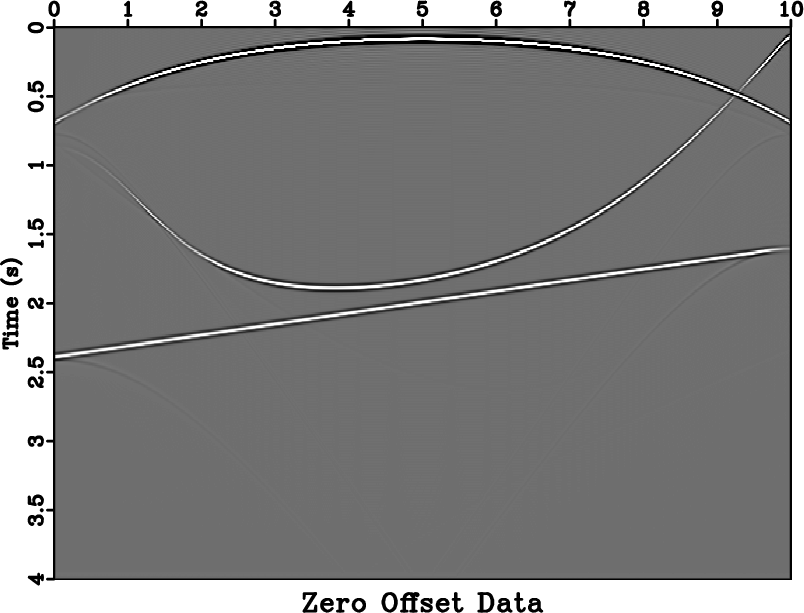
\includegraphics[scale=0.3]{./pic/report_april/Figure_4.png}
}
\captionof{figure}{ZO-сейсмограмма для модели с тремя отражающими горизонтами.}
\label{seismo_4}
\end{minipage}

\subsection{Миграция. Интеграл Кирхгофа.}

Рассмотрим простейший случай, когда расчётная сетка кубическая, и на поверхности сейсмоприёмники расположены в каждом её узле.
В таком случае формула (\ref{rayleigh_migration}) может быть записана в виде:
\begin{equation}
\label{rayleigh_migration_discrete}
U^m(i,j,k) = -\frac{1}{2\pi}\frac{\sum\limits_{l,m} \frac{U(l,m,\frac{2d(i,j,k+1,l,m)}{c})}{d(i,j,k+1,l,m)}\delta x \delta y - \sum\limits_{l,m} \frac{U(l,m,\frac{2d(i,j,k,l,m)}{c})}{d(i,j,k,l,m)}\delta x \delta y}{\delta z},
\end{equation}
где $d(i,j,k,l,m)=\sqrt{(l-i)^2(\delta x)^2 + (m-j)^2(\delta y)^2  + (k)^2(\delta z)^2}$, а начало координат находится в точке $(i,j,k)=(0,0,0)$.

Была реализована программа AcInverse на языке C++, производящая миграцию Кирхгофа (Рэлея).
Для её тестирования были использованы сейсмограммы, генерируемые ПО Madagascar для различного расположения отражающих границ.
Во всех задачах для удобства фиксировались следующие параметры: фоновая скорость распространения продольных волн 2500 м/с, геометрия расчётной области 10 км x 5 км,
временная функция источника - Риккер с основной частотой 25 Гц, измерительная система - 2001 источник и 2001 приёмник, установленные каждые 5 м.
При миграции шаг сетки составлял 5 x 5 м.

На рисунках (\ref{seismo_verif_model_0} - \ref{seismo_verif_model_3}) представлены ZO-сейсмограммы и миграционные изображения, рассчитанные в AcInverse.
Рассматрились четыре различные постановки задачи (отличаются формой границ):
\begin{itemize}
\item $z = -2$ и $z = -2 + (0.1 * x + 0.5)$
\item $z = -1$ и $z = -2$
\item $z = -1.5 - \frac{(x - 5)^2}{25}$ и $z = -1 - \frac{(x - 5)^2}{25}$
\item $z = -1.2 - sin(\frac{(x-5)^2}{2})$ и $z = -0.2 - sin(\frac{(x-5)^2}{2})$
\end{itemize}

\noindent
\begin{minipage}{\linewidth}
\makebox[\linewidth]{
\begin{tabular}{cc}
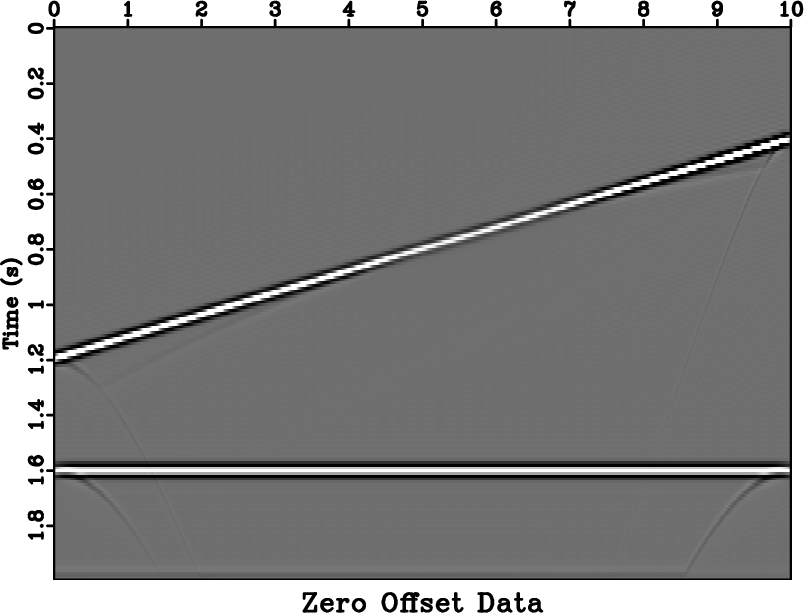
\includegraphics[width=50mm]{./pic/report_april/zodata_0.png}
&
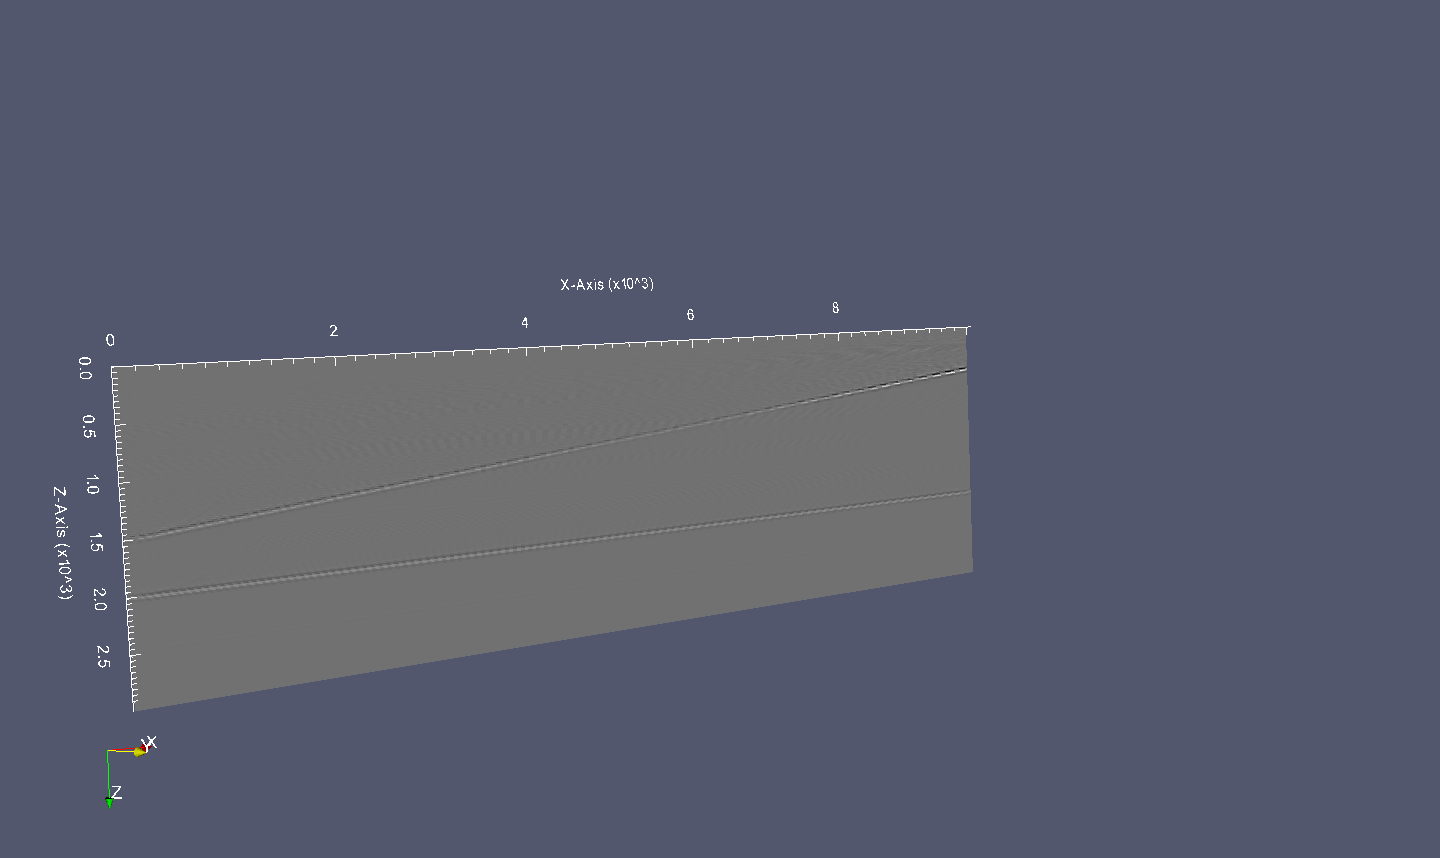
\includegraphics[width=60mm]{./pic/report_april/model_0.png}
\end{tabular}
}
\captionof{figure}{ZO-сейсмограмма (слева) и миграционное изображение справа. Модель 0.}
\label{seismo_verif_model_0}
\end{minipage}

\noindent
\begin{minipage}{\linewidth}
\makebox[\linewidth]{
\begin{tabular}{cc}
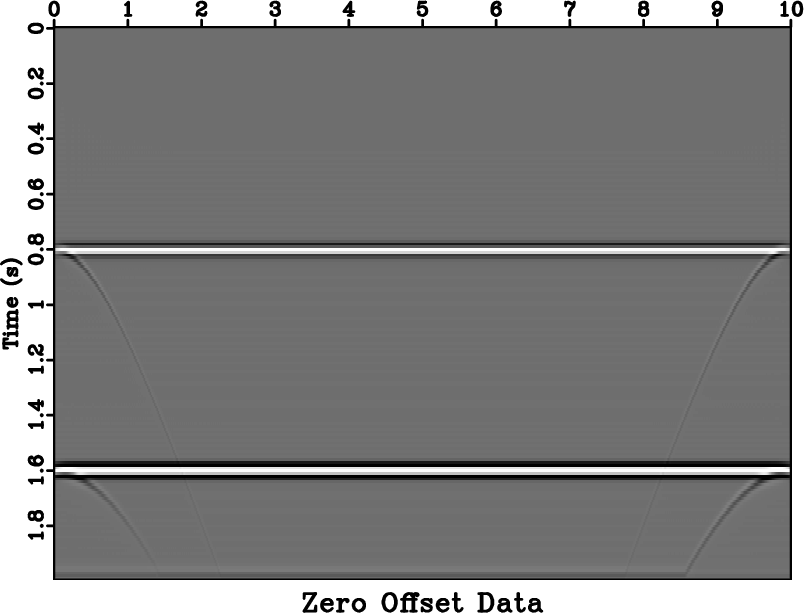
\includegraphics[width=50mm]{./pic/report_april/zodata_1.png}
&
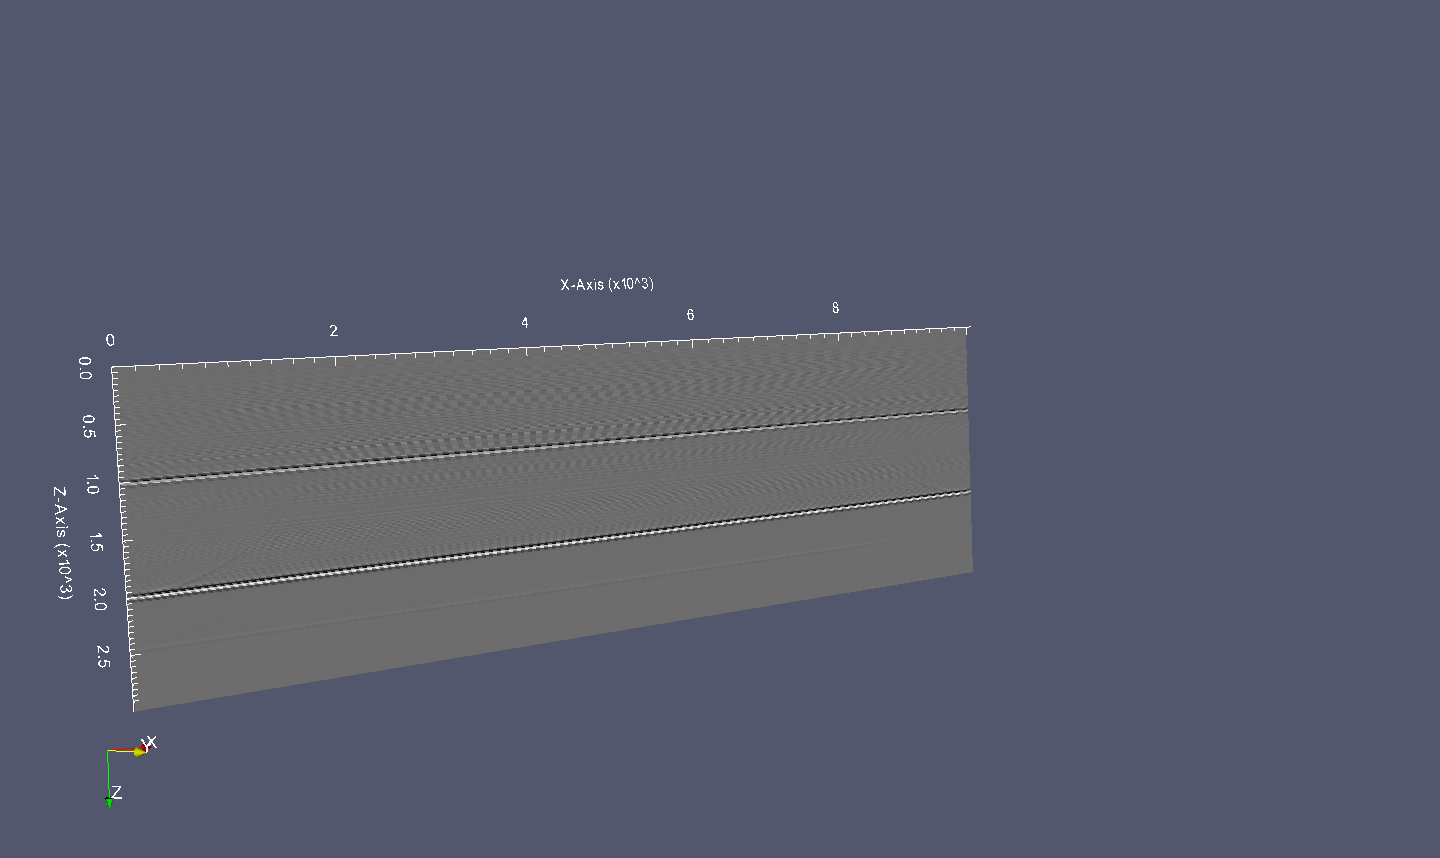
\includegraphics[width=60mm]{./pic/report_april/model_1.png}
\end{tabular}
}
\captionof{figure}{ZO-сейсмограмма (слева) и миграционное изображение справа. Модель 1.}
\label{seismo_verif_model_1}
\end{minipage}

\noindent
\begin{minipage}{\linewidth}
\makebox[\linewidth]{
\begin{tabular}{cc}
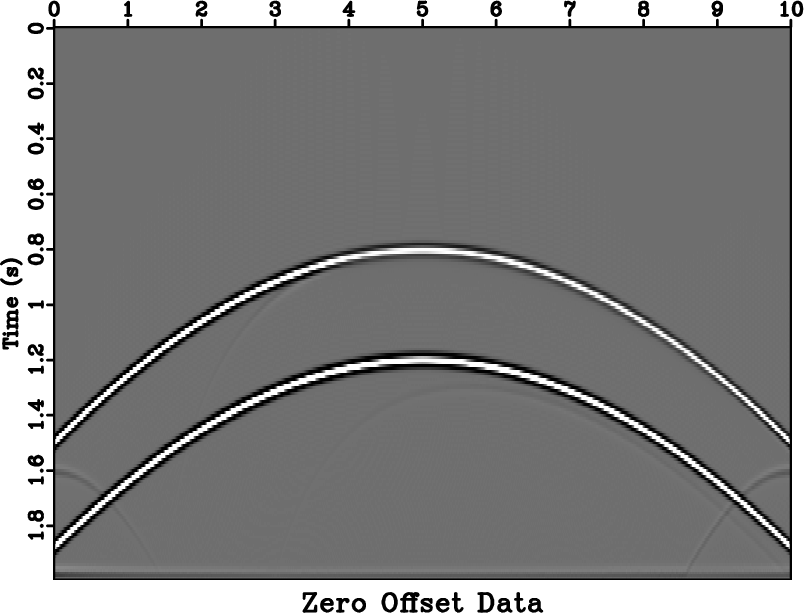
\includegraphics[width=50mm]{./pic/report_april/zodata_2.png}
&
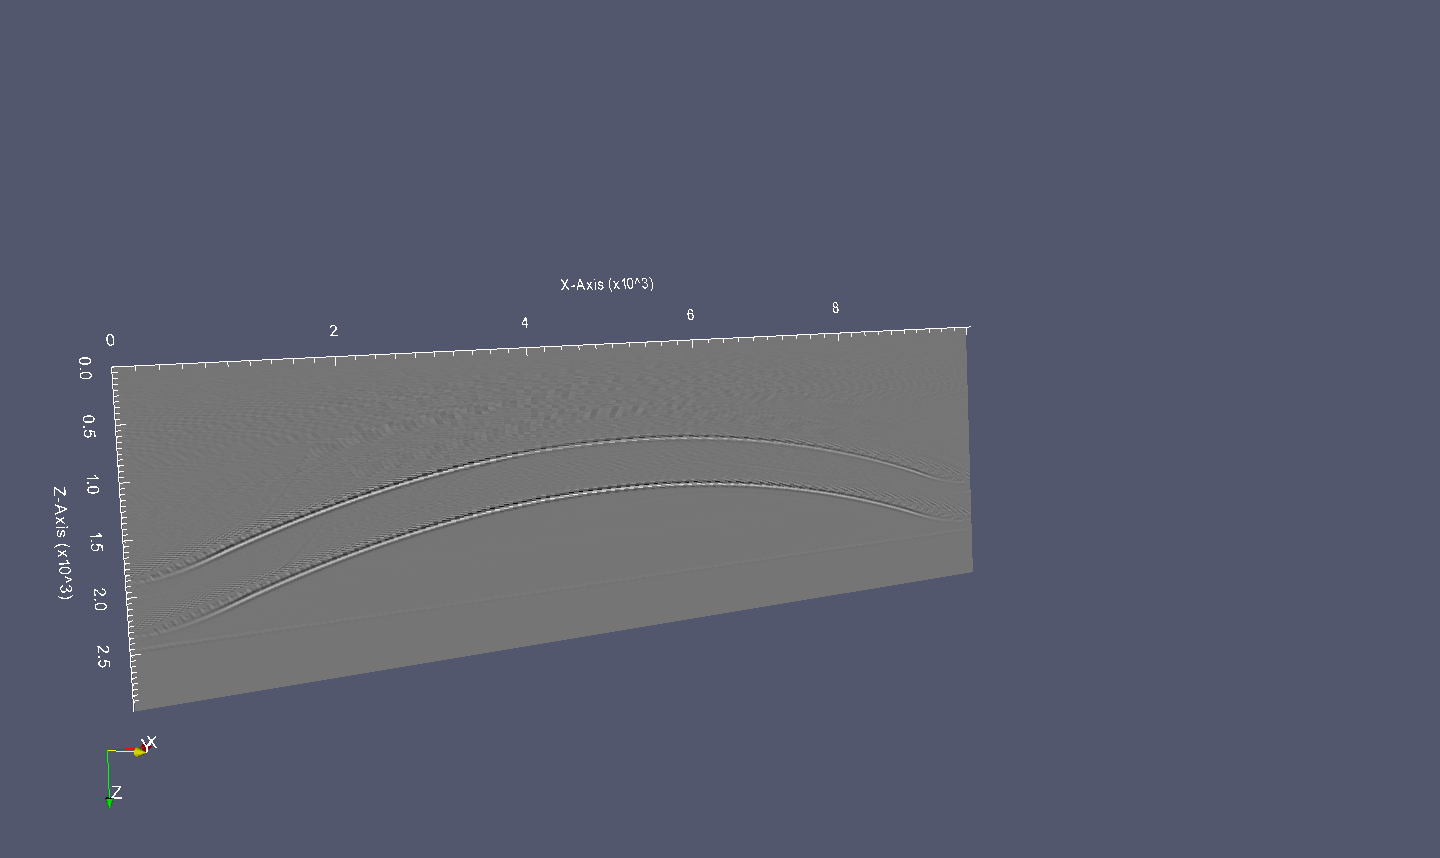
\includegraphics[width=60mm]{./pic/report_april/model_2.png}
\end{tabular}
}
\captionof{figure}{ZO-сейсмограмма (слева) и миграционное изображение справа. Модель 2.}
\label{seismo_verif_model_2}
\end{minipage}

\noindent
\begin{minipage}{\linewidth}
\makebox[\linewidth]{
\begin{tabular}{cc}
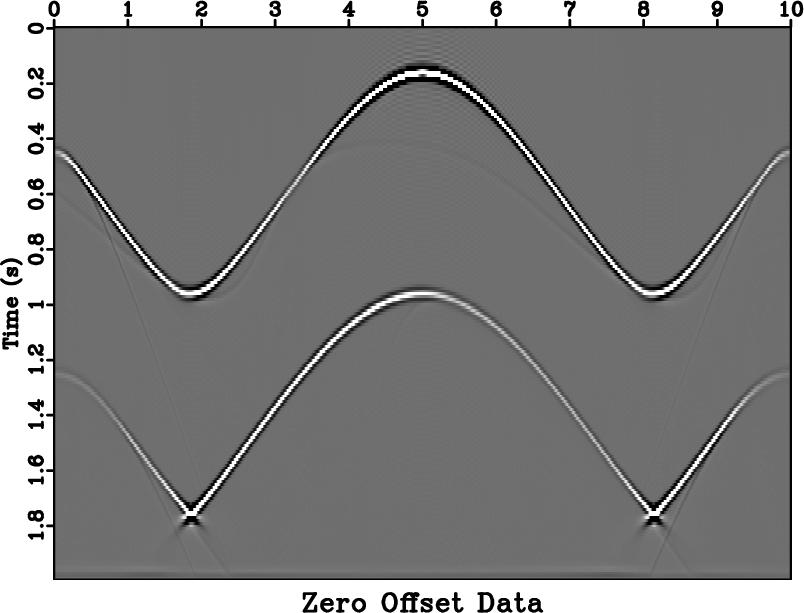
\includegraphics[width=50mm]{./pic/report_april/zodata_3.png}
&
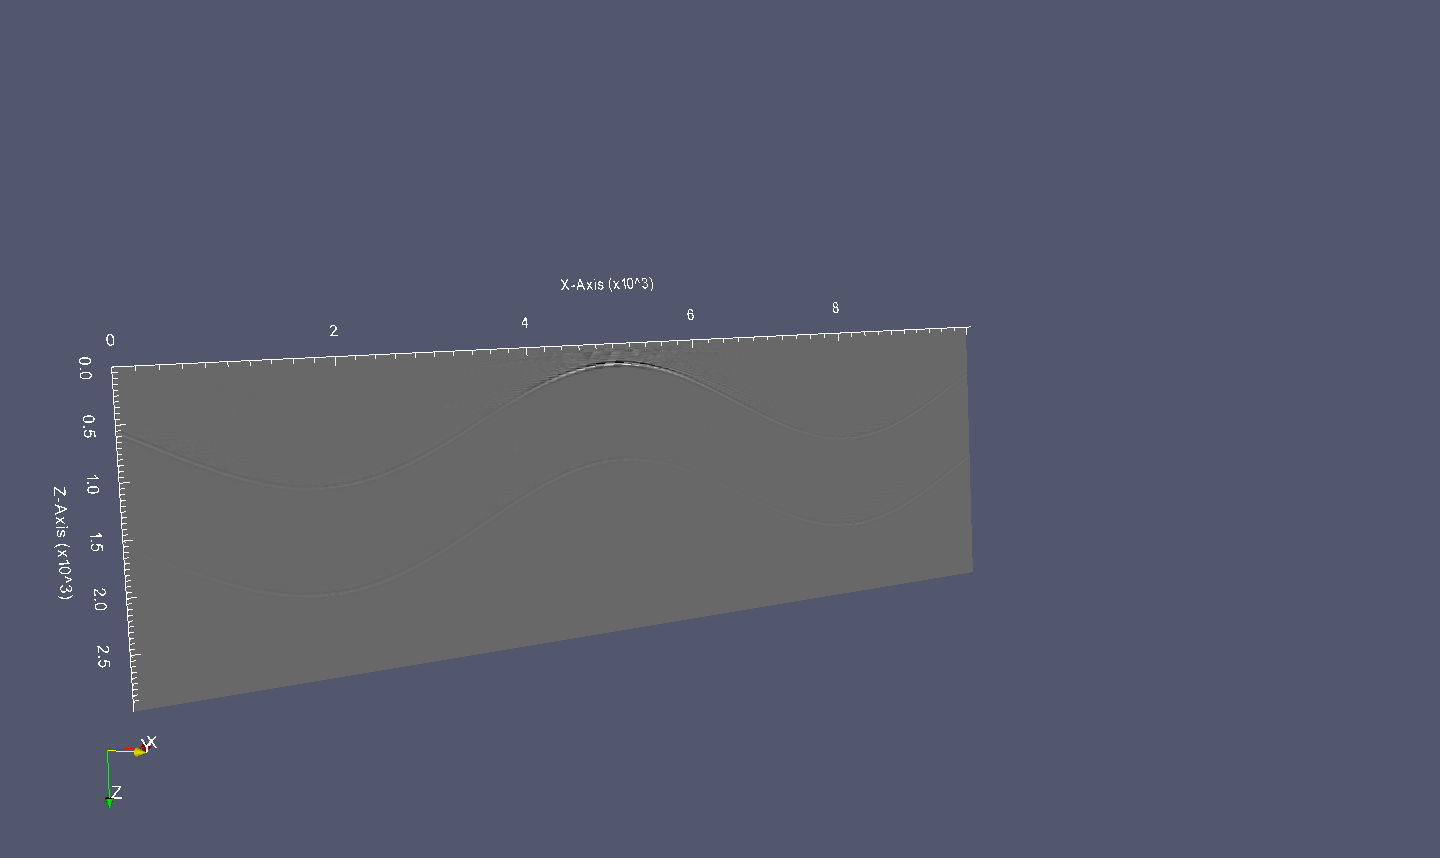
\includegraphics[width=60mm]{./pic/report_april/model_3.png}
\end{tabular}
}
\captionof{figure}{ZO-сейсмограмма (слева) и миграционное изображение справа. Модель 3.}
\label{seismo_verif_model_3}
\end{minipage}

\subsection{Миграция. Приближение Борна.}

Была разработана программа на языке \emph{C++}.
Решение уравнения \eqref{m_0} производилось методом \emph{BiCGSTAB}, реализованным в библиотеке \emph{PETSc}.
Интегрирование в формулах (\ref{th_1}-\ref{th_2}) производилось методом прямоугольников:
\begin{equation} \label{L}
\fun_L(\vR,t|\vr) \fun_m(\vr) = \sum_{\vr} \frac{ f_M^2 }{ 2 \left( \rmR \right)^2 } e^{ -\tau^2 } \left( \tau^4 - 3 \tau^2 + \frac{3}{4} \right) \fun_m(\vr) \Delta V ,
\end{equation}
\begin{equation} \label{LT}
\fun_L^*(\vR|\vr,t) \fun_d(\vr, t) = \sum_{t} \sum_{\vr} \frac{ f_M^2 }{ 2 \left( \rmR \right)^2 } e^{ -\tau^2 } \left( \tau^4 - 3 \tau^2 + \frac{3}{4} \right) \fun_d(\vr,t) \Delta S \Delta t .
\end{equation}
Запуск программы осуществлялся на ноутбуке \emph{Samsung RC530} с процессором \emph{Intel Core i7-2670QM}. 

В качестве контрольной модели среды была использована двумерная модель \emph{Marmousi} \cite{marmousi}. Она основана на геологической структуре морского дна у берегов Анголы и является классическим примером сложной акустической модели, используемой для тестирования вычислительных алгоритмов сейсмической миграции. Распределение медленности в данной модели изображено на \figref{marmousi}.
\begin{figure}[tb]
\centering
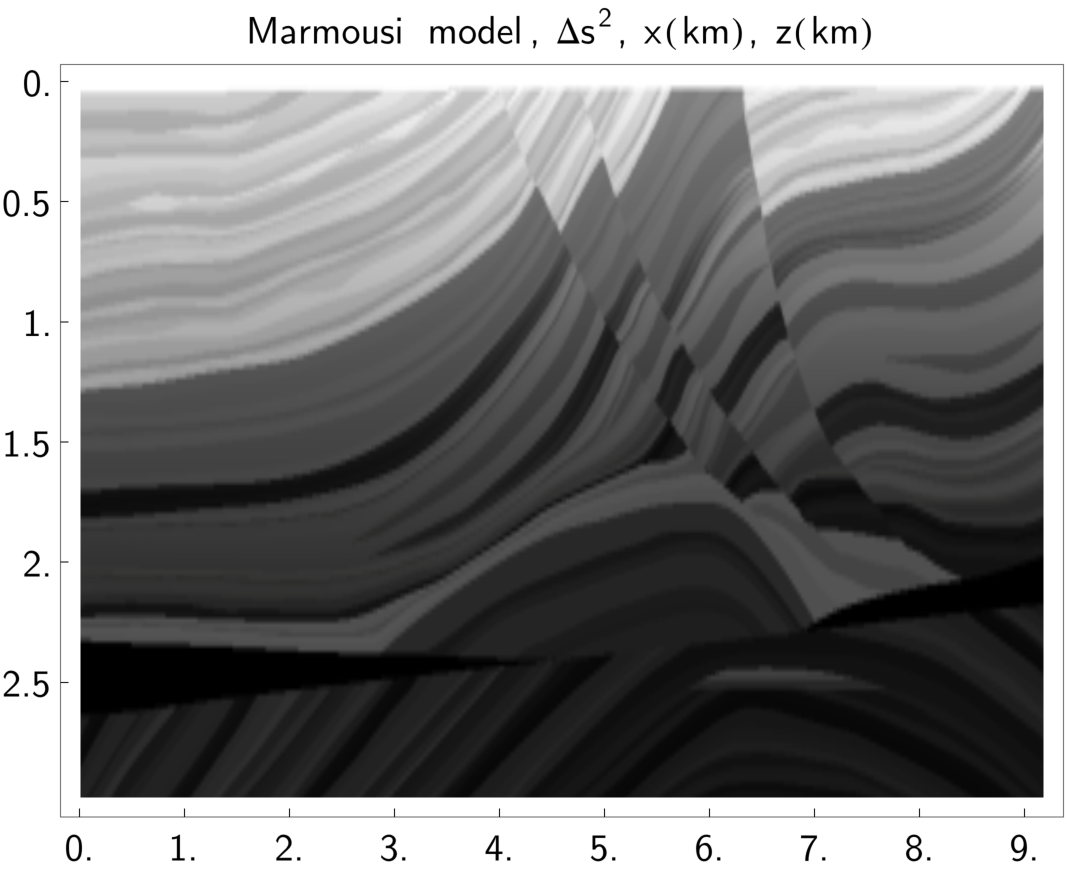
\includegraphics[width=.5\textwidth]{pic/report_april/marmousi}
\caption{Модель Marmousi}\label{marmousi}
\end{figure}

В качестве входных данных для построения миграционных изображений использовались сейсмограммы, полученные с помощью \eqref{L}. Приемники располагались на поверхности $z = 0$ на одинаковых расстояниях друг от друга $X_i = X_{min} + i\Delta X$. Отсчеты по времени производились через равные промежутки $t_i = t_{min} + i\Delta t$.

Обозначим \begin{itemize}
\item число приемников $n_X$                                     
\item положение первого приемника $X_{min}$ в метрах             
\item расстояние между соседними приемниками $\Delta X$ в метрах 
\item число отсчетов по времени $n_t$                            
\item начальное время $t_{min}$ в секундах                       
\item шаг по времени $\Delta t$ в секундах
\item общее число значений данных $N = n_X \times n_t$                   
\item положение первого узла расчетной сетки $(x,z)$ в метрах    
\item шаг расчетной сетки $\Delta x \times \Delta z$ в метрах    
\item число узлов расчетной сетки $M = n_X \times n_z$
\end{itemize}

Значения этих параметров для каждого расчета приведены в следующей таблице:
\begin{center} \begin{tabular}{|c|c|c|c|c|} \hline
Номер расчета              & $1$                 & $2 $                & $3$                   & $4$                   \\ \hline
$n_X$                      & $115$               & $115$               & $460$                 & $240$                 \\ \hline
$X_{min}$                  & $40$                & $40$                & $10$                  & $2575$                \\ \hline
$\Delta X$                 & $80$                & $80$                & $20$                  & $25$                  \\ \hline
$n_t$                      & $200$               & $100$               & $190$                 & $190$                 \\ \hline
$t_{min}$                  & $0$                 & $1$                 & $0.125$               & $0.125$               \\ \hline
$\Delta t$                 & $0.01$              & $0.01$              & $0.0125$              & $0.0125$              \\ \hline
$N = n_Xn_t$               & $23000$             & $11500$             & $87400$               & $45600$               \\ \hline
$(x,z)$                    & $(40,20)$           & $(40,20)$           & $(10,10)$             & $(0,8)$               \\ \hline
$\Delta x \times \Delta z$ & $80\times 40$       & $80\times 40$       & $20\times 20$         & $4\times 4$           \\ \hline
$M = n_X \times n_z$       & $115\times 75=8625$ & $115\times 75=8625$ & $460\times 150=69000$ & $2301\times 749=1723449$ \\ \hline
\end{tabular} \end{center}

Также зададим одинаковые для всех расчетов \begin{itemize}
\item несущую частоту для функции $RW(t)$ $f_M = 25$ Гц
\item и фоновую медленность $s_b = (3.5 \text{км}/\text{с})^{-1}$
\end{itemize}

\subsubsection{Нормализация}
Из вида выражения \eqref{L} можно сделать вывод, что участки сейсмограммы, соответствующие малым временам, будут "подсвечены" сильнее тех, которые соответствуют большим. Вследствие невысокого динамического диапазона окончательного изображения удобно при отображении его нормализовать. Следующая формула дает простой способ нормализации:
\begin{equation}
\fun_d_{norm}(\vr,t) = \frac{ \fun_d(\vr,t) } { \sum_{\vR} \fun_d(\vR,t) } .
\end{equation}
То же самое касается миграционного изображения: для него роль времени играет глубина.

\subsubsection{Расчёты на грубой сетке (1 и 2)}
Результаты первых двух расчетов изображены на \figref{marmresult1}, \figref{marmresult2}. В качестве входных данных второго расчета использована вторая половина сейсмограммы из первого расчета. Можно видеть, что модель среды, полученая в первом расчете, значительно хуже той, которая получена во втором, при сейсмограммах схожего качества.
%
\begin{figure}[tb]
\centering
\begin{subfigure}{.3333\textwidth}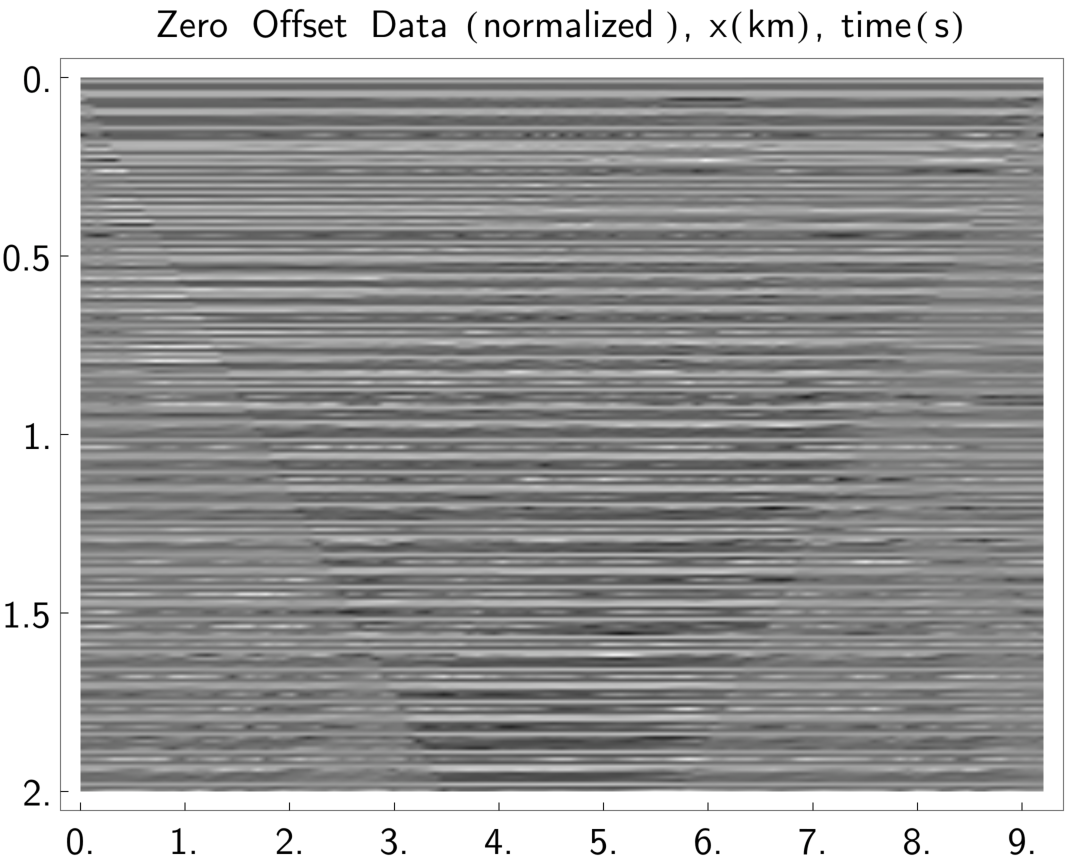
\includegraphics[width=\textwidth]{pic/report_april/zo_seism_toobad_norm}\caption{сейсмограмма}\end{subfigure}%
\begin{subfigure}{.3333\textwidth}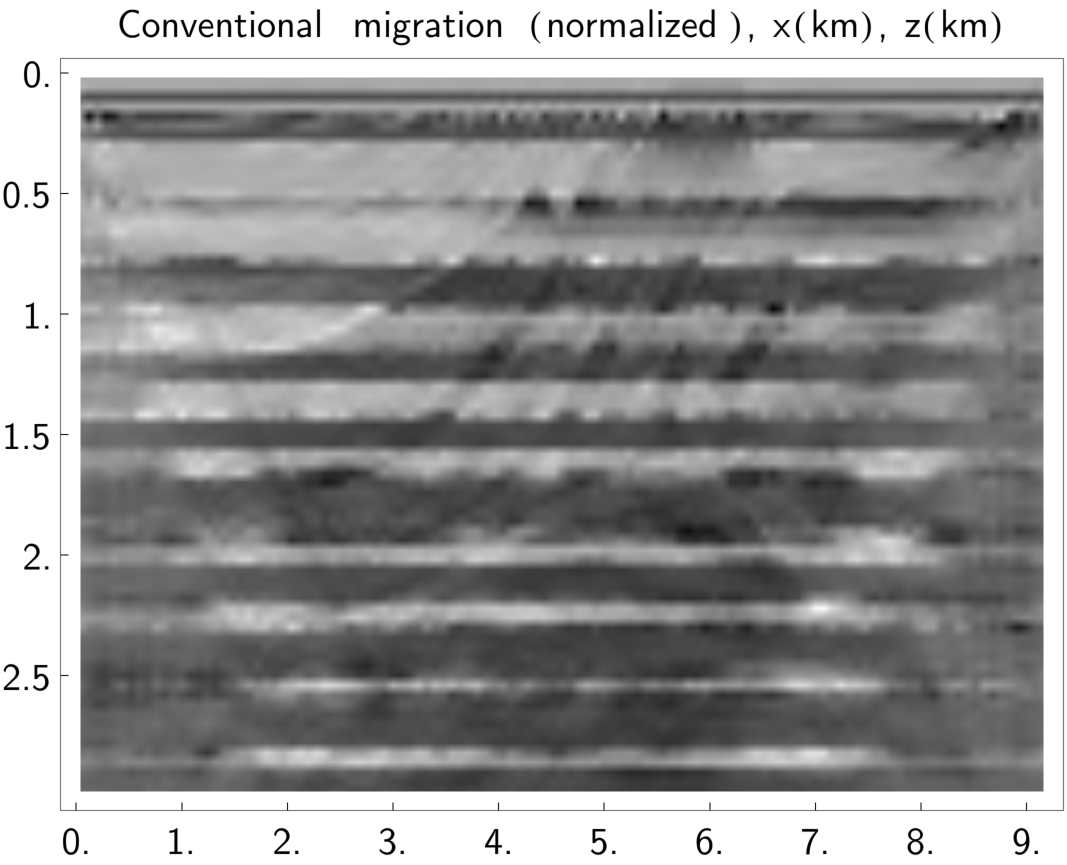
\includegraphics[width=\textwidth]{pic/report_april/zo_migr_toobad_norm}\caption{миграционное изображение}\end{subfigure}%
\begin{subfigure}{.3333\textwidth}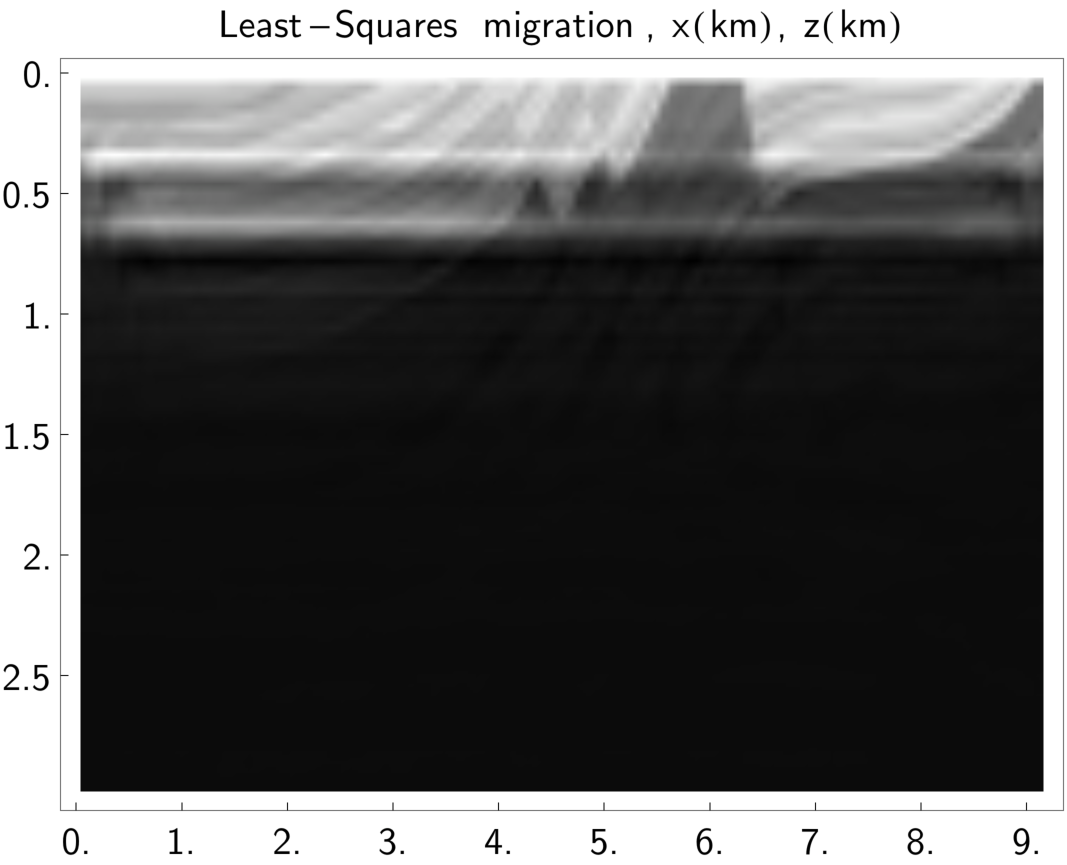
\includegraphics[width=\textwidth]{pic/report_april/zo_inv_toobad}\caption{полученная модель среды}\end{subfigure}%
\caption{Результаты первого расчета} \label{marmresult1}
\end{figure}
%
\begin{figure}[tb]
\centering
\begin{subfigure}{.3333\textwidth}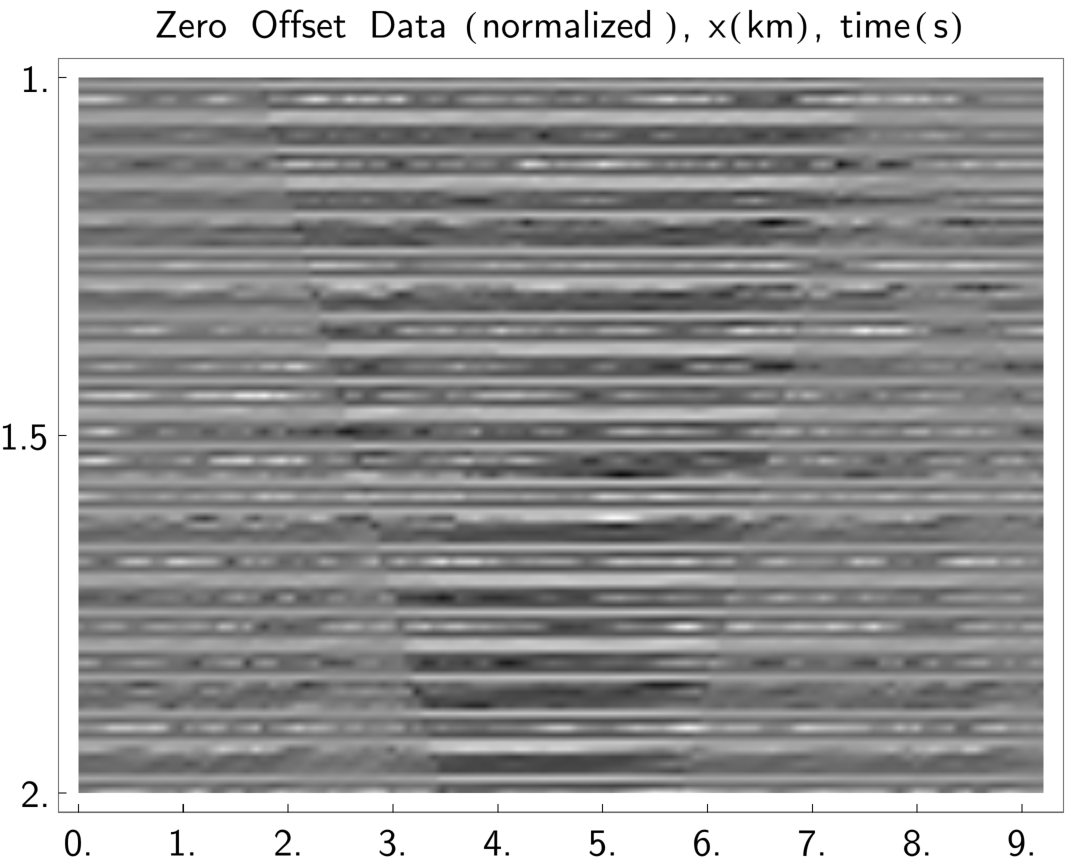
\includegraphics[width=\textwidth]{pic/report_april/zo_seism_bad_norm}\caption{сейсмограмма}\end{subfigure}%
\begin{subfigure}{.3333\textwidth}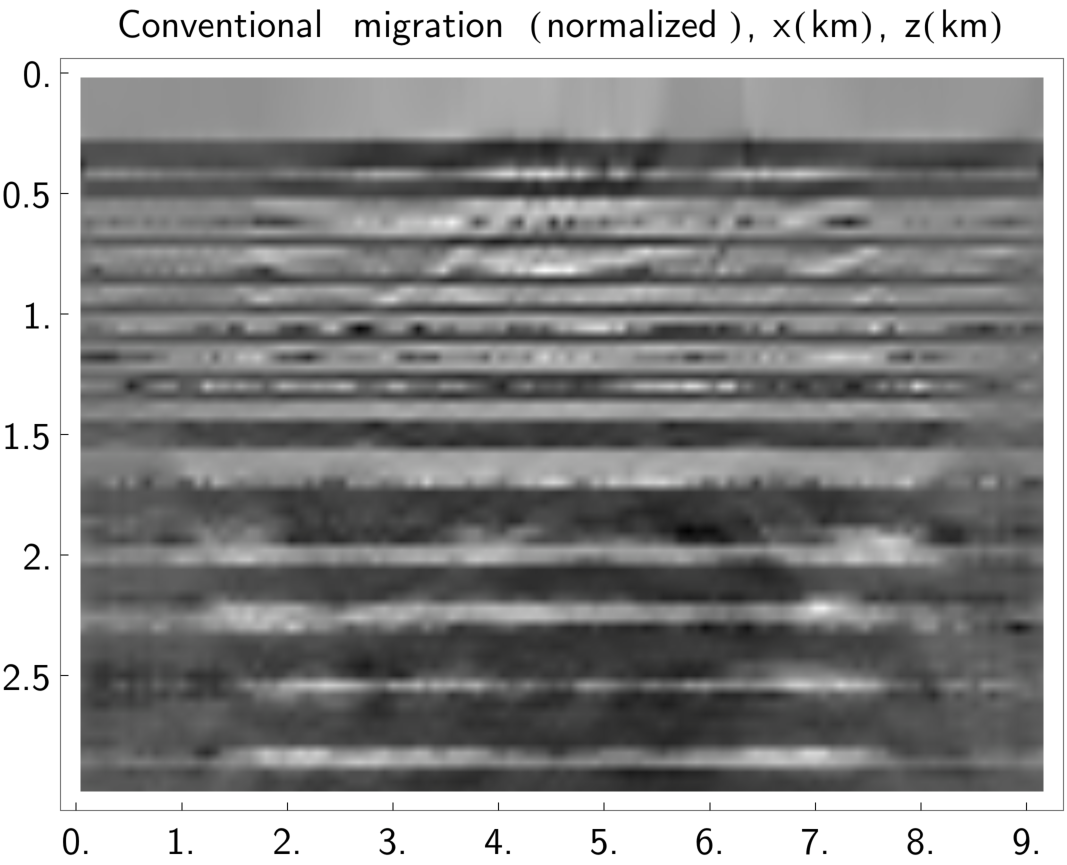
\includegraphics[width=\textwidth]{pic/report_april/zo_migr_bad_norm}\caption{миграционное изображение}\end{subfigure}%
\begin{subfigure}{.3333\textwidth}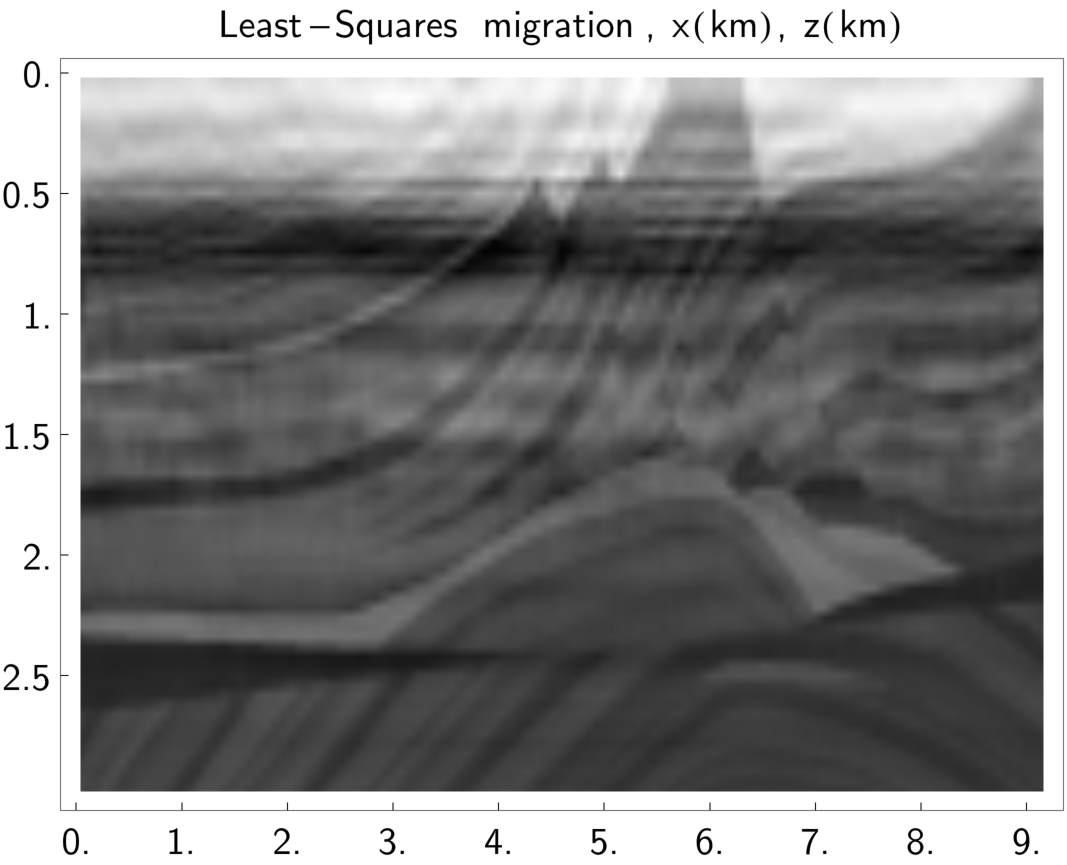
\includegraphics[width=\textwidth]{pic/report_april/zo_inv_bad}\caption{полученная модель среды}\end{subfigure}%
\caption{Результаты второго расчета} \label{marmresult2}
\end{figure}
%
Ненормализованная сейсмограммы изображены на \figref{marmresult12}. По ним можно сделать вывод, что низкое качество полученной модели в первом расчете обусловлено высоким разбросом абсолютных значений сейсмоданных в первой половине сейсмограммы.
%
\begin{figure}[tb]
\centering
\begin{subfigure}{.3333\textwidth}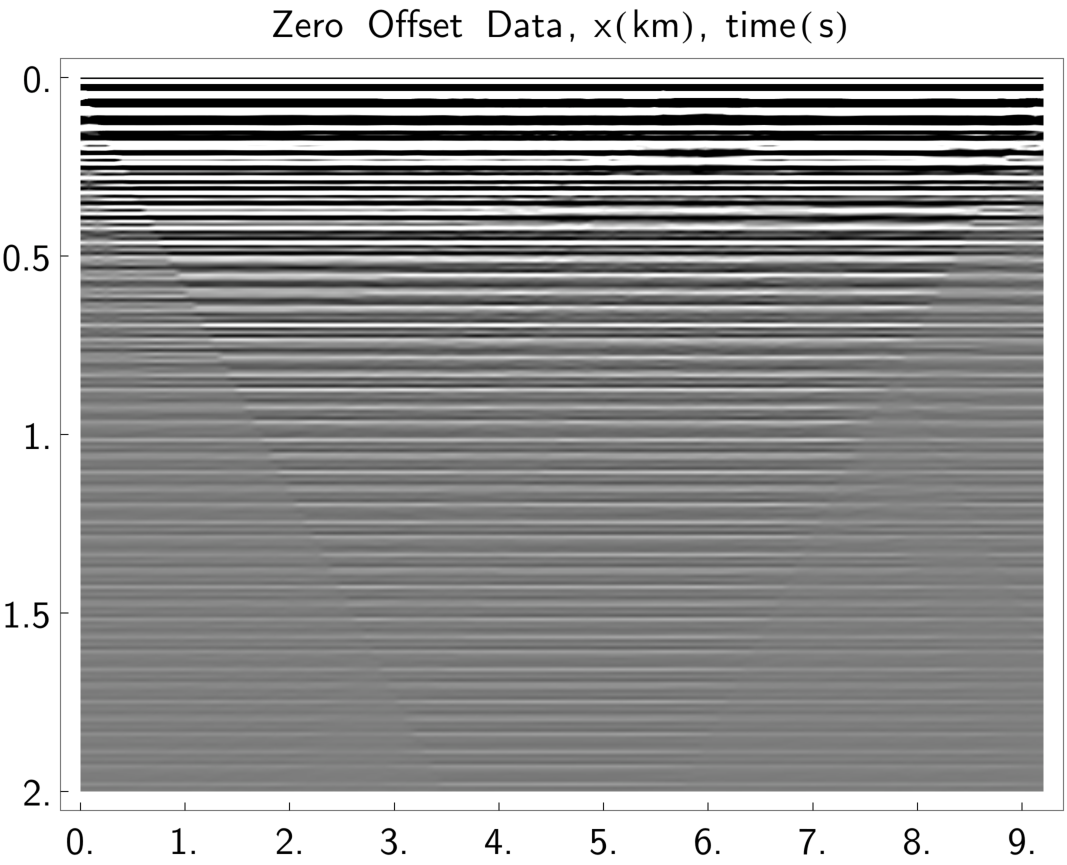
\includegraphics[width=\textwidth]{pic/report_april/zo_seism_toobad}\caption{первый расчет}\end{subfigure}\hspace{.1111\textwidth}
\begin{subfigure}{.3333\textwidth}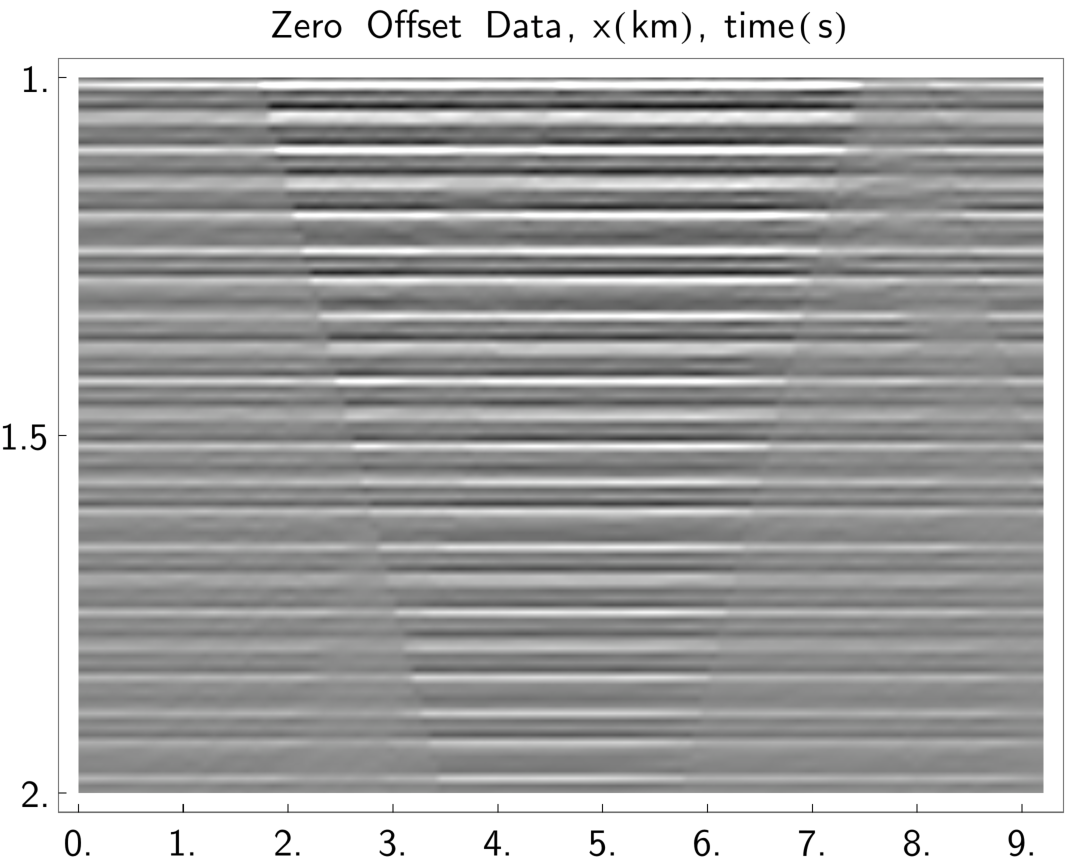
\includegraphics[width=\textwidth]{pic/report_april/zo_seism_bad}\caption{второй расчет}\end{subfigure}%
\caption{Ненормализованные сейсмограммы первого и второго расчетов} \label{marmresult12}
\end{figure}

Низкое качество сейсмограмм, а с ними и миграционных изображений, в данных расчетах обусловлено большим шагом сетки.
Расчет показывает, что при данных параметрах шаг сетки не должен привышать $20$ метров \figrefp{step}.
%
\begin{figure}[tb]
\centering
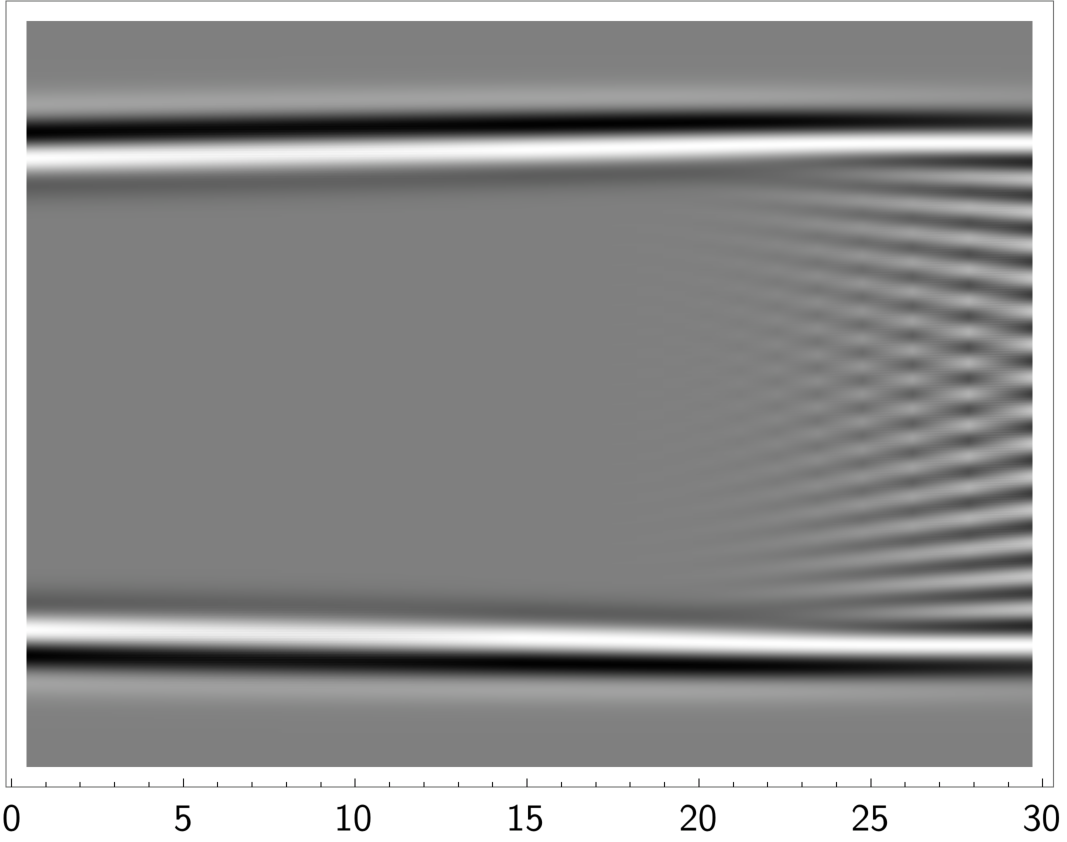
\includegraphics[width=.3333\textwidth]{pic/report_april/step}
\caption{Изменение изображения элементарного слоя (425 м) на сейсмограмме с ростом шага сетки (в метрах)}\label{step}
\end{figure}

\subsubsection{Расчёт на мелкой сетке (3)}
Результаты расчета 3 представлены на \figref{marmresult3}. В данном расчете по сравнению с первыми двумя шаг сетки уменьшен до $20$ метров по обоим направлениям. Расстояние между приемниками также уменьшено до $20$-ти метров. При данных параметрах произвести расчет по формуле \eqref{m_0} на имеющемся оборудовании не представляется возможным. В то же время традиционная миграция дает приемлимый результат.
%
\begin{figure}[tb]
\centering
\begin{subfigure}{.5\textwidth}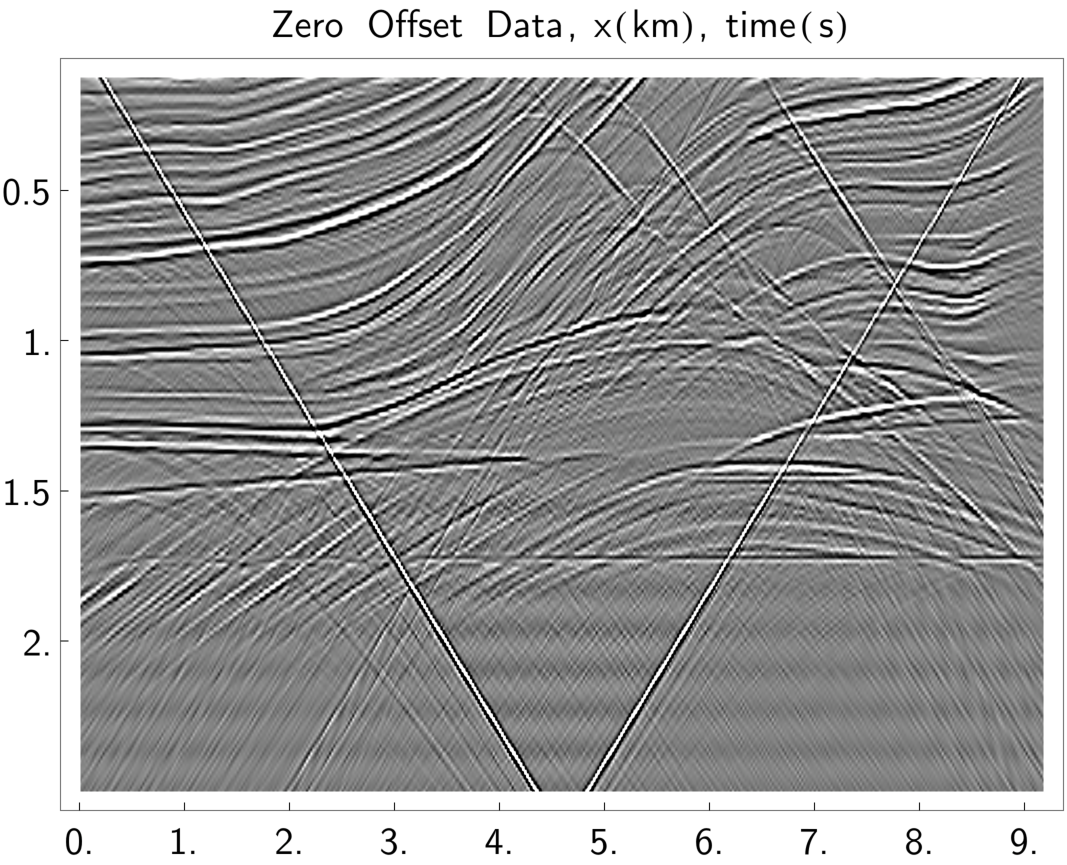
\includegraphics[width=\textwidth]{pic/report_april/zo_seism_good_norm}\caption{сейсмограмма}\end{subfigure}%
\begin{subfigure}{.5\textwidth}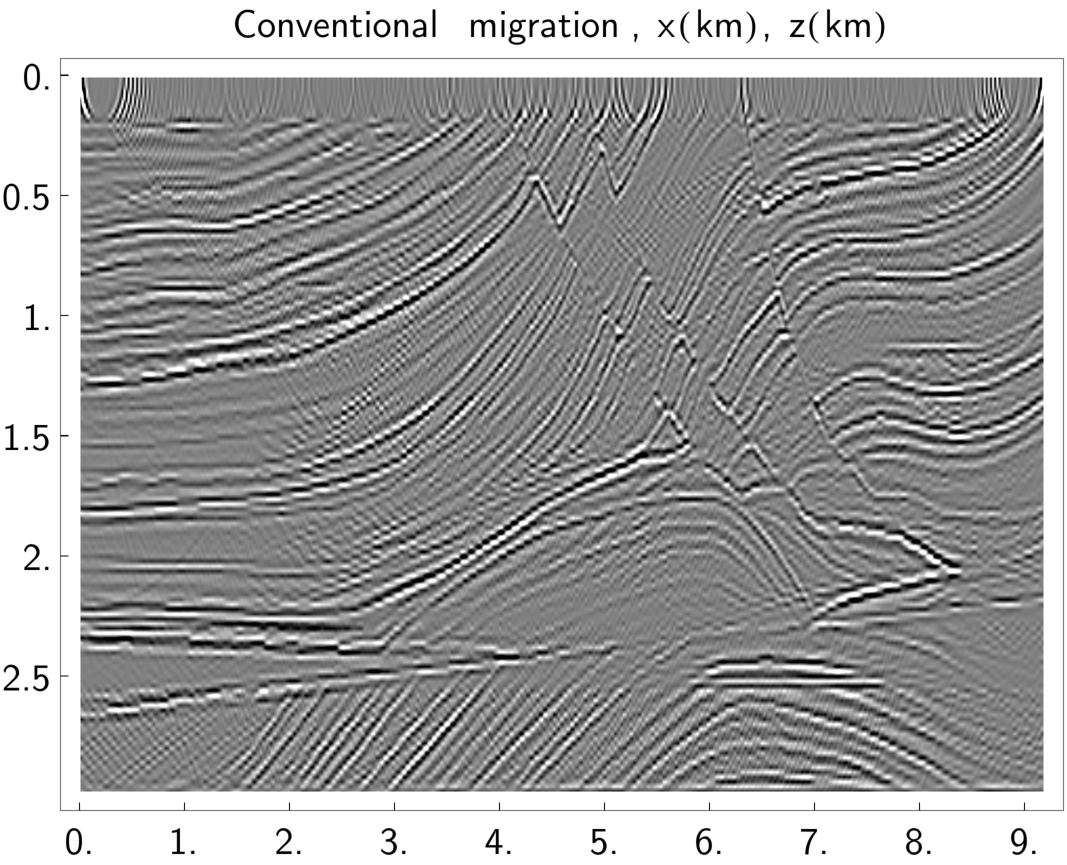
\includegraphics[width=\textwidth]{pic/report_april/zo_migr_good_norm}\caption{миграционное изображение}\end{subfigure}%
\caption{Результаты третьего расчета} \label{marmresult3}
\end{figure}

\subsubsection{Сравнение с синтетическими данными (4)}
В заключение приведем сравнение сейсмограммы, полученной в результате расчета 4, с сейсмограммой, представленной в \cite{marmousi} \figrefp{marmresult4}. Расчет производился для удаления источника возмущения на $425$ метров вправо от приемника ("near-offset"). Напомним, что приближение Борна корректно при условии малости отраженного от неоднородности среды поля по сравнению с фоновым полем. В случае рассматриваемой модели это условие не выполняется. Некорректность используемого приближения проявляется в том, что на полученной сейсмограмме каждый слой с постоянной медленностью получается растянут или сжат относительно образца соответственно отклонению медленности в нем от фоновой. Другими словами, границы слоев на изображении модели можно совместить с границами слоев на полученной сейсмограмме, если отмасштабировать время на последней на половину фоновой скорости (см. выражение для $\tau$ в \eqref{eq:13}), в то время как для сейсмограммы-образца так сделать нельзя.

Миграционное изображение среды, полученное в результате расчета 4 представлено на \figref{marmresult4b}
%
\begin{figure}[tb]
\centering
\begin{subfigure}{.5\textwidth}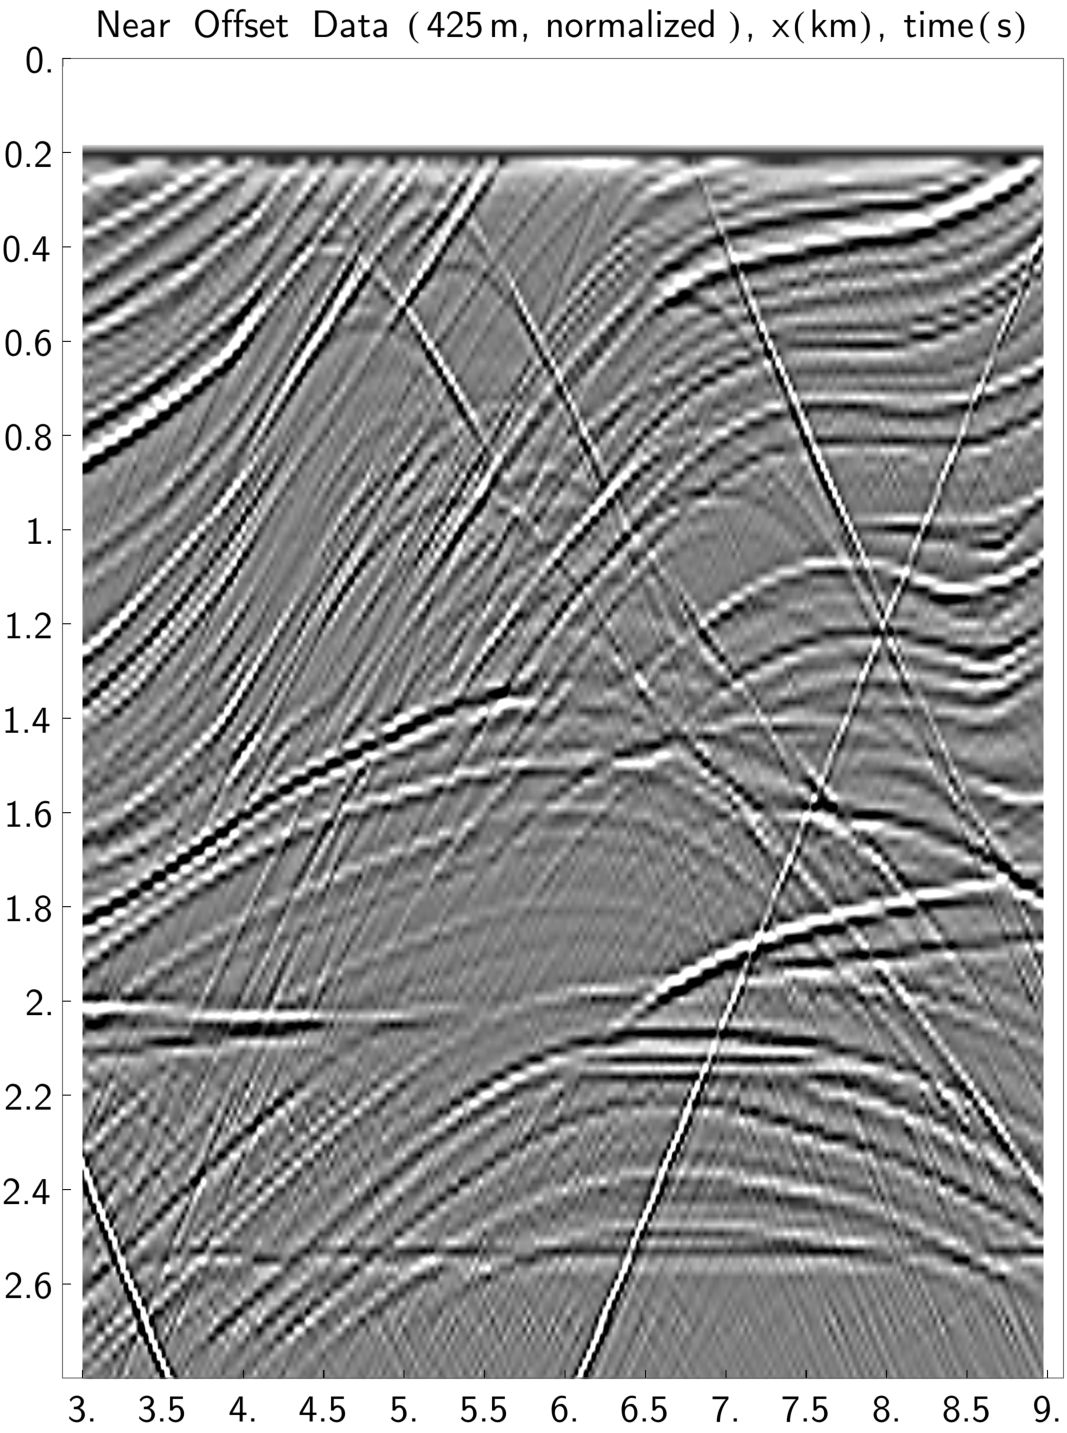
\includegraphics[width=\textwidth]{pic/report_april/no_seism_norm}\end{subfigure}%
\begin{subfigure}{.5\textwidth}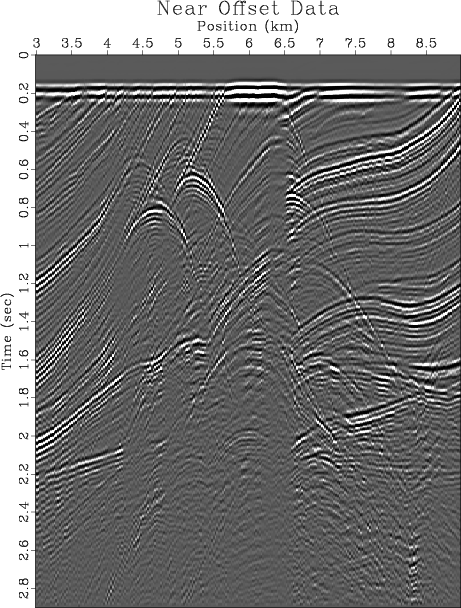
\includegraphics[width=\textwidth,trim=0 0 0 2cm]{pic/report_april/nearOffset}\end{subfigure}%
\caption{Сравнение сейсмограммы, полученной в результате четвёртого расчета (слева), и сейсмограммы-образца (справа)} \label{marmresult4}
\end{figure}
%
\begin{figure}[tb]
\centering
\begin{subfigure}{.5\textwidth}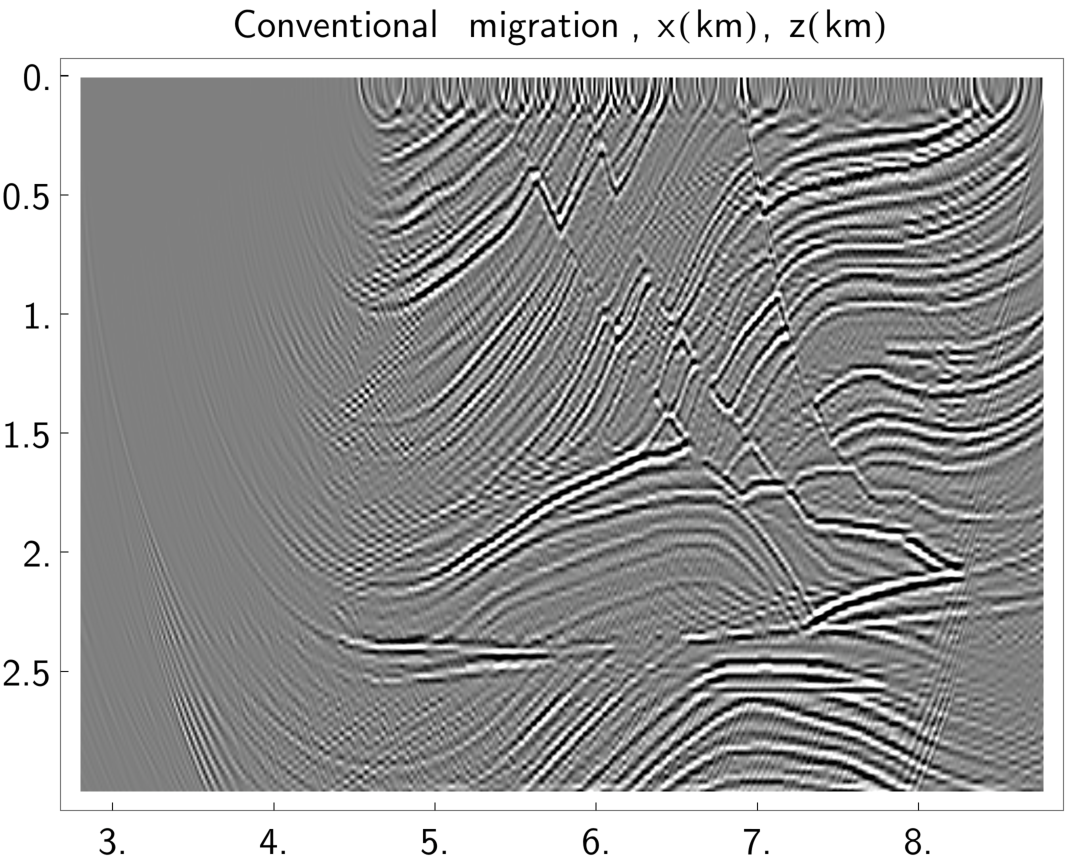
\includegraphics[width=\textwidth,trim=0 0 0 2cm]{pic/report_april/no_migr_norm}\end{subfigure}%
\begin{subfigure}{.5\textwidth}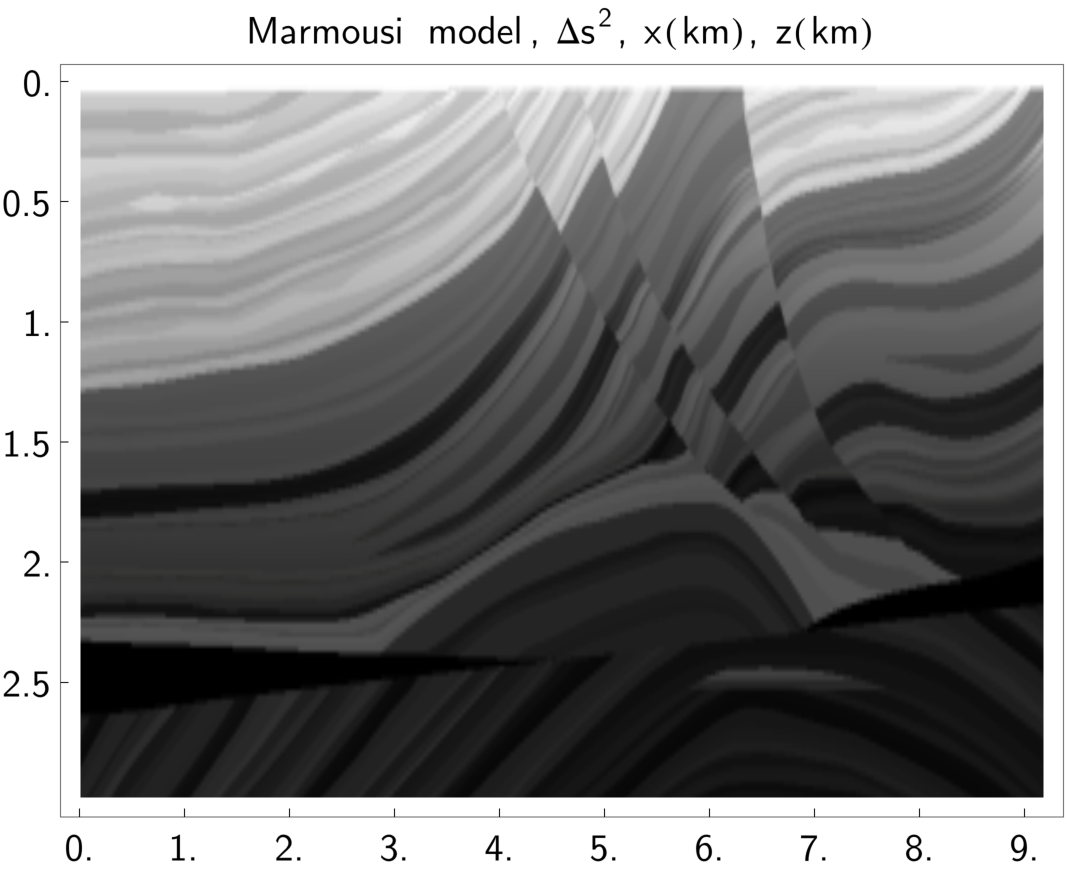
\includegraphics[width=\textwidth,trim=0 0 0 2cm]{pic/report_april/marmousi}\end{subfigure}%
\caption{Миграционное изображение, полученное в результате четвёртого расчета (слева) и модель (справа)} \label{marmresult4b}
\end{figure}

\subsection{Сравнительный анализ двух алгоритмов миграции (Кирхгоф, Борн) на простых моделях}

Одной из целей работы являлось сравнение двух методов миграции (Кирхгоф и присоединённый оператор), реализованных в программах AcInverse и Borni.
Исследовалась 2D модель с двумя отражающими горизонтами\footnote{При расчёте сейсмограммы в Borni отражающие границы образовывались как результат включения одной большой неоднородности с $\delta s = 4*10^{-6}$}, которые задавались формулами:
\begin{itemize}
\item $z=-2$,
\item $z=-2 + (0.1 * x + 0.5)$.
\end{itemize}
Фоновая скорость распространения продольных волн 2500 м/с, геометрия расчётной области 10 км x 5 км.
Временная функция источника - Риккер с основной частотой 25 Гц.
В измерительную систему входил 201 источник и 201 приёмник, установленные каждые 50 м.

На рисунке \ref{seismo_verif_zo_madagascar_borni} (слева) приведена Zero-Offset-сейсмограмма, рассчитанная методом Кирхгофа (Madagascar, kirmod), а справа - программой Borni.
Как видно, Кирхгоф дал более чёткое изображение, хотя и с наличием сферических артефактов у границ области.
Таким образом, для тестирования алгоритмов миграции было получено два набора входных данных разными методами.

\noindent
\begin{minipage}{\linewidth}
\makebox[\linewidth]{
\begin{tabular}{cc}
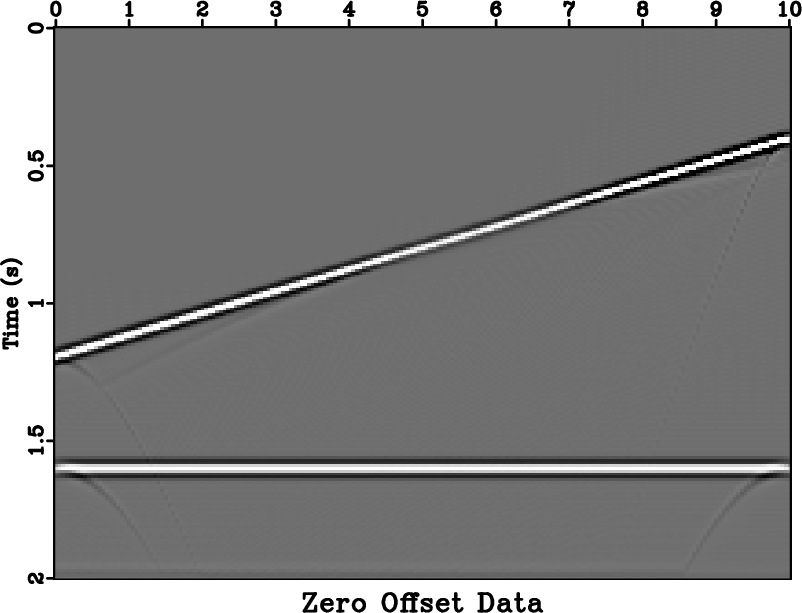
\includegraphics[width=50mm]{./pic/report_april/seismo_verif_zo_madagascar_borni-madagascar.png}
&
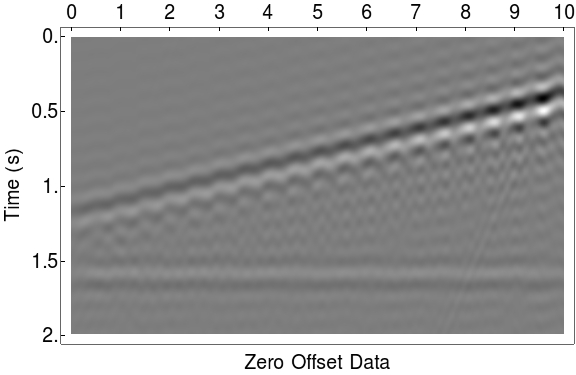
\includegraphics[width=60mm]{./pic/report_april/seismo_verif_zo_madagascar_borni-borni.png}
\end{tabular}
}
\captionof{figure}{ZO-сейсмограмма для верификационной модели. Слева - Madagascar, справа - Borni.}
\label{seismo_verif_zo_madagascar_borni}
\end{minipage}

На рисунке \ref{seismo_verif_madagascar_borni-acinverse} представлены миграционные изображения, полученные методом Кирхгофа (AcInverse).
Можно говорить о выделяемости контактных границ, пусть и с небольшим контрастом и наличием артефактов.

\noindent
\begin{minipage}{\linewidth}
\makebox[\linewidth]{
  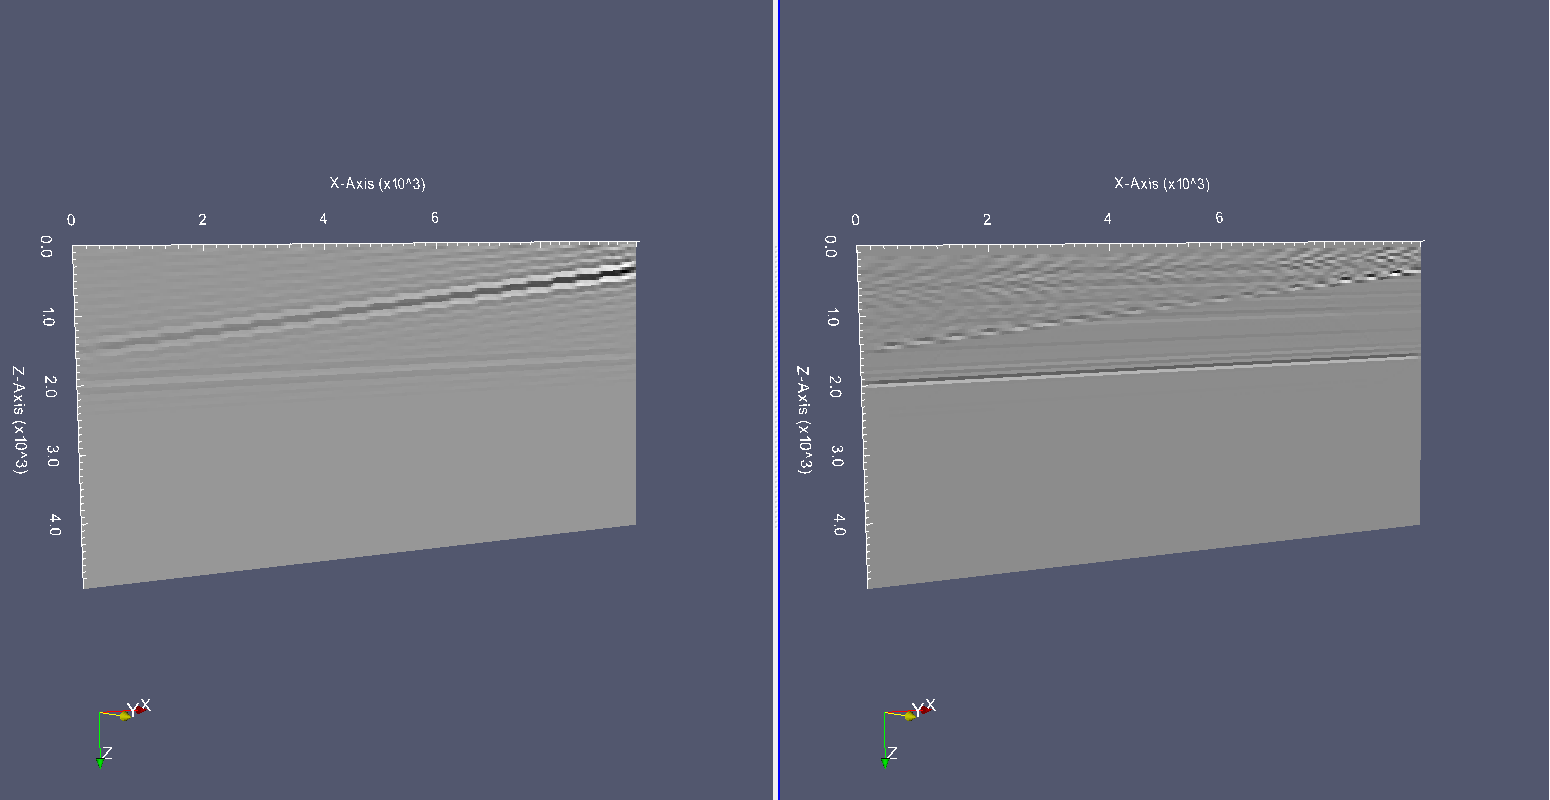
\includegraphics[width=100mm]{./pic/report_april/seismo_verif_madagascar_borni-acinverse.png}
}
\captionof{figure}{Миграционное изображение для верификационной модели, полученное методом Кирхгофа (AcInverse). Слева - на входе Борн (Borni), справа - на входе Кирхгоф (Madagascar).}
\label{seismo_verif_madagascar_borni-acinverse}
\end{minipage}

На рисунке \ref{seismo_verif_madagascar_borni-borni} представлены миграционные изображения, полученные методом присоединённого оператора (Борн, Borni).

\noindent
\begin{minipage}{\linewidth}
\makebox[\linewidth]{
  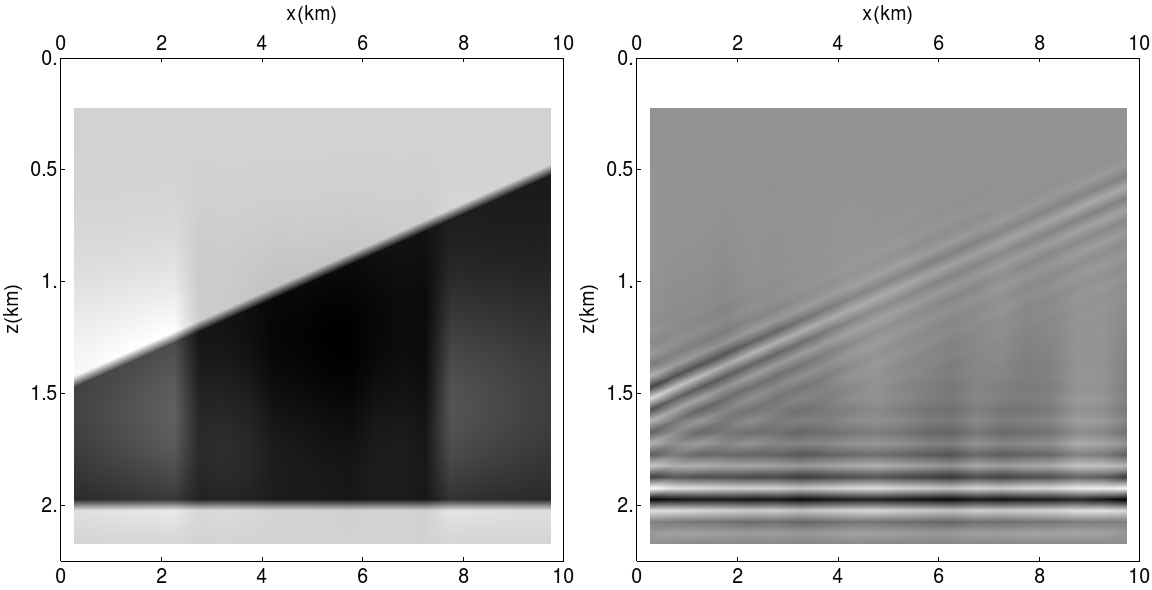
\includegraphics[width=120mm]{./pic/report_april/seismo_verif_madagascar_borni-borni.png}
}
\captionof{figure}{Миграционное изображение для верификационной модели, полученное методом присоединённого оператора (Борн, Borni). Слева - на входе Борн (Borni), справа - на входе Кирхгоф (Madagascar).}
\label{seismo_verif_madagascar_borni-borni}
\end{minipage}

\section{Заключение}

Таким образом, к настоящему моменту разработаны программы, позволяющие проводить процедуру миграции по алгоритмам Кирхгофа и Борна.
Также имеется возможность решения прямой задачи (построения синтетических сейсмограмм) на основе интеграла Кирхгофа и приближения Борна.

Алгоритм миграции Кирхгофа протестирован на слоистых моделях с криволинейными границами.
Нужно отметить, что в зависимости от расчётной геометрии наблюдается значительное расхождение в "выделяемости" отражающих границ на миграционном изображении.

Алгоритм миграции Борна протестирован на модели Marmousi, характеризующейся сложной геометрией.
Показано, что при использовании достаточно мелкой расчётной сетки могут быть восстановлены параметры модели.
Однако, не решён вопрос с "размытием" синтетической сейсмограммы и миграционного изображения из-за некорректности описания сложной модели в виде background + small difference.
Также вычислительная сложность алгоритма получилась чрезвычайно высокой, что требует отдельного осмысления.

Выполнено сравнение результатов "построение синтетической сейсмограммы" $-$ "миграция" для программ AcInverse и Borni на слоистой модели.

Возможные направления дальнейшего исследованияания: 

\begin{enumerate}
\item Провести детальное исследование поведения алгоритмов миграции (AcInverse, Borni) при изменении расчётных параметров.
\item Провести верификационные сравнения таким же способом (К-К, Б-Б, К-Б, Б-К) на 2Д слоистых моделях с криволинейными границами, т.о. усложнив "простые модели".
\item Освоить в Madagascar решение прямой задачи FD методом (или доработать сеточно-характеристический метод), получить синтетическую ZO-сейсмограмму от верификационной трёхслойной модели и попробовать применить миграцию AcInverse и Borni.
\item Продлить границы 2Д модели вдоль третьей оси, чтобы получить 3Д, и провести верификационное тестирование на полученной 3Д модели.
\item Освоить Madagascar с целью построения ZO-сейсмограммы для сложной модели (например, Marmousi) и попробовать применить миграцию AcInverse и Borni.
\item Доработать Borni для реализации regularized least-square migration.
\item Перейти к построению матрицы L на основе finite-difference approximation, а потом реализовать аналог Borni на её основе.
\item Провести параллелизацию Borni и AcInverse для ускорения расчётов.
\end{enumerate}

\section{Приложение 1. Пример построения матрицы L в приближении Борна}

Согласно теории, изложенной в \cite{Zhdanov_2007}, в акустическом приближении связь между наблюдаемым давлением на
сейсмоприёмниках на поверхности и параметрами среды может быть выражена следующей формулой (приближение Борна, \cite{Zhdanov_2007}, 15.5):

\begin{equation}
\label{eq_born_approximation_1}
p^s(\vec{r}_j, w) = w^2\int_D G^w_b(\vec{r}_j|\vec{r};w)\Delta s^2(\vec{r})p^i(\vec{r},w)  dv,
\end{equation}

в которой $\vec{r}_j$ - радиус-вектор точки приёмника, $D$ - область, в которой параметр медленности ($s = \frac{1}{c}$)
отличается от фоновой медленности ($s_b = \frac{1}{c_b},\Delta s^2 = \frac{1}{c^2} - \frac{1}{c^2_b})$, $p^i$ - давление, которое создавалось бы
в отсутствии неоднородности в области $D$, $G^w_b$ - функция Грина для фоновой медленности.
Для однородной среды функция Грина может быть записана в виде (\ref{eq_grin_function}).
Подставляя (\ref{eq_grin_function}) в формулу (\ref{eq_born_approximation_1}) получим:

\begin{equation}
\label{eq_born_approximation_2}
p^s(\vec{r}_j, w) = w^2\int_D \frac{1}{4\pi|\vec{r}-\vec{r}_j|}e^{iw\frac{|\vec{r}-\vec{r}_j|}{c_b}} \Delta s^2(\vec{r})p^i(\vec{r},w)  dv.
\end{equation}

Займёмся теперь вычислением $p^i$.
Пусть источник возмущения - точечный взрыв, происходящий в нулевой момент времени в точке $\vec{r}_0$.
Тогда в случае однородной среды с фоновой медленностью $s_b$ можно записать решение в виде:

\begin{equation}
\label{eq_point_explosion}
p^i(\vec{r}, w) = \frac{1}{4\pi|\vec{r}-\vec{r}_0|}e^{iw\frac{|\vec{r}-\vec{r}_0|}{c_b}}.
\end{equation}

Подставляя (\ref{eq_point_explosion}) в формулу (\ref{eq_born_approximation_2}) получим:

\begin{eqnarray}
\label{eq_born_approximation_3}
p^s(\vec{r}_j, w) = w^2\int_D \frac{1}{4\pi|\vec{r}-\vec{r}_j|}e^{iw\frac{|\vec{r}-\vec{r}_j|}{c_b}} \Delta s^2(\vec{r})\frac{1}{4\pi|\vec{r}-\vec{r}_0|}e^{iw\frac{|\vec{r}-\vec{r}_0|}{c_b}}  dv = \nonumber \\
= \frac{w^2}{16\pi^2} \int_D \frac{e^{iw\frac{|\vec{r}-\vec{r}_0| + |\vec{r}-\vec{r}_j|}{c_b}}}{|\vec{r}-\vec{r}_j||\vec{r}-\vec{r}_0|} \Delta s^2(\vec{r}) dv.
\end{eqnarray}

Вводя дискретизацию по пространству в виде параллелепипедной сетки с шагами $\delta x, \delta y, \delta z$ и индексами $l, m, p$ формулу (\ref{eq_born_approximation_3}) можно
привести к виду:

\begin{equation}
\label{eq_born_approximation_num}
p^s(\vec{r}_j, w) = \frac{w^2}{16\pi^2} \sum_{(l,m,p)\in D} \frac{e^{iw\frac{|\vec{r}_{l,m,p}-\vec{r}_0| + |\vec{r}_{l,m,p}-\vec{r}_j|}{c_b}}}{|\vec{r}_{l,m,p}-\vec{r}_j||\vec{r}_{l,m,p}-\vec{r}_0|} \Delta s_{l,m,p}^2 \delta x \delta y \delta z.
\end{equation}

На первом этапе рассмотрим двумерный случай, когда вдоль $Y$ содержится всего одна ячейка.
Тогда можно избавиться от индекса $m$, а также сейсмодатчики устанавливаются вдоль одной линии $OX$ и могут быть параметризованы одним индексом $j$.
Формула (\ref{eq_born_approximation_num}) сводится к виду:

\begin{equation}
\label{eq_born_approximation_num_2D}
p^s(x_j, w) = \frac{w^2 \delta x \delta z}{16\pi^2} \sum_{(l,p)\in D} \frac{e^{iw\frac{D_{l,p}+d_{j,l,p}}{c_b}}}{D_{l,p}d_{j,l,p}} \Delta s_{l,p}^2,
\end{equation}

где $D_{l,p}=|\vec{r}_{l,p}-\vec{r}_0|$ и $d_{j,l,p}=|\vec{r}_{l,p}-\vec{x}_j|$.

Пусть матрица $\Delta s_{l,p}^2$ развернута в $1D$ массив так, что последовательно в нём лежат её строки.
И пусть размер модели по $X$ равен $P$, а по $Z$ - $L$.
Тогда индекс в массиве имеет вид $ind = p + l * P$, $p \in [0, P - 1], l \in [0, L - 1]$.
Также справедливы равенства: $l = [\frac{ind}{P}]$ и $p = ind - [\frac{ind}{P}] * P$.

С учётом введённой параметризации массива и того факта, что вне неоднородности $\Delta s^2 = 0$, можно записать формулу (\ref{eq_born_approximation_num_2D}) в виде:

\begin{equation}
\label{eq_born_approximation_num_2D_ind}
p^s(x_j, w) = \sum_{(ind)\in [0, L * P - 1]} L_{j,ind} \Delta s_{ind}^2,
\end{equation}

где матрица $L_{j,ind} = \frac{w^2 \delta x \delta z}{16\pi^2} \frac{e^{iw\frac{D_{ind}+d_{j,ind}}{c_b}}}{D_{ind}d_{j,ind}}$,
$D_{ind}=\sqrt{(x_{ind} - x_0)^2 + (y_{ind} - y_0)^2}$ и $d_{j,ind}=\sqrt{(x_{ind} - x_j)^2 + y_{ind}^2}$.
Это и является реализованным представлением зависимости данных на приёмниках от параметров модели.
При обобщении на трёхмерный случай усложнится лишь формула для вычисления значения $ind$, тогда как все остальные рассуждения не изменятся.

\bibliographystyle{acm}
\bibliography{report_April_1}

\end{document}
